% Delete the MSc option if you are doing a PhD, or replace it with MPhil
% for a Master of Philosophy thesis
%
% The 12pt option is required by the 2001/02 thesis regulations
% Last update 15th August 2007: new Abstract format and Copyright Statement

% Replace MSc with PhD for PhD theses
% Remove the twoside option for single-sided printing
\documentclass[12pt,MSc,a4paper,oneside]{muthesis}
\usepackage[a4paper]{geometry} % It saves some pages
\usepackage[utf8]{inputenc}
\usepackage{algorithmic}
\usepackage[chapter]{algorithm}
\usepackage{hyperref}
\usepackage{url}
\usepackage{svg}
\usepackage{listings}
\usepackage{tabularx}
\usepackage{ltablex}
\usepackage{xltabular}
\hypersetup{
    colorlinks=true,       % false: boxed links; true: colored links
    linkcolor=black,          % color of internal links
    citecolor=black,        % color of links to bibliography
    filecolor=black,      % color of file links
    urlcolor=blue           % color of external links
}
\usepackage{amsmath,amssymb}
\usepackage[authoryear,colon]{natbib}
\usepackage{xspace}
\usepackage{booktabs}
\usepackage{graphicx}
\graphicspath{ {./images/} }

\newcommand{\detailtexcount}[1]{%
  \immediate\write18{texcount -merge -sum #1.tex > #1.wcdetail }%
  \verbatiminput{#1.wcdetail}%
}
 
\newcommand{\quickwordcount}[1]{%
  \immediate\write18{texcount -1 -sum -merge #1.tex > #1-words.sum }%
  \input{#1-words.sum} words%
}
 
\newcommand{\quickcharcount}[1]{%
  \immediate\write18{texcount -1 -sum -merge -char #1.tex > #1-chars.sum }%
  \input{#1-chars.sum} characters (not including spaces)%
}

% \oddsidemargin 5truemm \evensidemargin -8truemm
% \marginparwidth 40pt \marginparsep 10pt
% \topmargin -11.5truemm \headsep 7truemm
% \textheight 245truemm \textwidth 154truemm

\newcommand{\assign}{\ensuremath{=}}

\begin{document}

\begin{figure}[t]
\centering

\includegraphics[scale=0.1]{images/uom.png}
\end{figure}

\title{Forecasting Risk Factor Topics
Importance from financial reports}
\author{
Anusca Popa Ioan Armand 
\newline
Supervisor: Dr. Goran Nenadic
}
% \author{103}
\school{Department of Computer Science}
\faculty{Computer Science}

% Don't count these!
%%TC:ignore
\def\wordcount{\quickwordcount{main}}
%\quickcharcount{main}
%\detailtexcount{main}
%%TC:endignore


% Uncomment the line below to suppress the `List of Tables' page (optional)
%\tablespagefalse

% Uncomment the line below to suppress the `List of Figures' page (optional)
%\figurespagefalse

% Uncomment the line below to use a customised Declaration statement
% \def\declaration{}

%\maketitle
 
\beforeabstract


This project proposes a framework for a Natural Language Processing pipeline for extracting topics from financial documents and predicting their importance for future timestamps. It utilises annual statements from the U.S. Securities and Exchange Commission's database(SEC). These documents represent the picture companies drew, for their investors and the larger public, of the last year. They embedded critical financial data in the vocabulary used. The section used for this analysis is entitled Risk Factors. In this section, companies must disclose any foreseeable dangers to the entity's evolution. The dataset used in this project contains the annual statements from all the companies listed in the Central Index Key repository offered by SEC. The size of the dataset is approximately 30K spanning over 20 years. Both investors and business analysts widely use this to evaluate the market's attitude. 
The pipeline presented is an end to end solution for extracting, cleaning, preparing, processing and interpreting the results. It utilises data mining techniques, multiple pre-processing actions, BERTopic and a regression model to predict the importance of the extracted topics in the next year.
The methods used in the experiments are underlying a series of challenges that emerged in this field, proving there is value in combining them. The final results will predict how key topics might evolve in the future. From that dataset, the pipeline extracted 600 topics. For the most recent ones, it predicted their importance for the year 2021 with an absolute error of 1.41 points or an absolute percentage error of 35.96\%. These results can provide an insight into the overall state of the market and point towards main areas of development which should be followed closely by both investors and the larger public.

\afterabstract

% The next part is optional; however it is a good place to thank your
% supervisor and the people responsible for providing computer support ;-)
\prefacesection{Acknowledgements}
I want to express my gratitude to my supervisor, Dr Goran Nenadic, for sharing his expertise and supporting the development of this project.

% The next line is NOT optional and MUST appear
\afterpreface



\chapter{Introduction}

% This chapter covers the background material for my thesis and introduces
% the notation that I will use throughout.

\section{Motivation}
A document withholds relevant data for what it represents. That data is often hidden behind a form of unstructured text. Analysing data became a profitable domain as soon as our society started collecting it on a massive scale. However, analysing one document does not yield significant results. Data is generated at an unprecedented rate. It is becoming increasingly critical to every business. The context of that data also becomes crucial. We need to tackle more extensive datasets that offer a complete overview to model the context, but that requires time and resources.
Governmental bodies are asking for increased transparency from big corporations running in their countries, especially those holding considerable amounts of capital from investors: "All companies, foreign and domestic, are required to file registration statements, periodic reports, and other forms electronically. Through EDGAR."\cite{EDGAR}. That is being incorporated in quarterly and annual reports. They have to offer insights into all the aspects of a business. A big part of investing is minimising the risks.
Risk factors that affect or might affect a business are disclosed in a textual form. In this section of its report, companies disclose threats to their evolution in the coming years. The annual statements reports are one of the most valuable resources when performing business analysis. It provides a view of the performance of the company throughout the year. The format and structure of the reports mostly followed the same guidelines throughout the years. However, there is still a degree of liberty that every company utilises when filling these reports. They also embody a variety of legal and fiscal terms, which are hard to filter when manually analysing the documents. This reporting type is submitted by companies to U.S.Securities and Exchange Commission annually, outlining all aspects of the business. The essence of the reports represents a good source of data for multiple use cases, such as analysing trends for trading firms, law firms to train their employees in specific domains of expertise, or competing businesses to acknowledge and prepare for risks that might affect an entire industry.
For example, Apple stated in their 2017 report that: "The majority of the Companys research and development activities, its corporate headquarters, information technology systems, and other critical business operations, including certain component suppliers and manufacturing vendors, are in locations that could be affected by natural disasters."\cite{Apple201710K}. One interesting question from this statement is "What other companies have the same issue?" or more specifically "Where is that area that they describe as being critical for business operations such that can be affected by natural disasters?"
The project described in this report is aimed to create a framework that identifies and evaluates risks over a timeframe. The same objective would be a laborious task if undertaken manually. The way to move forwards is to automate it. That poses particular challenges such as data mining, information extraction, indexing and batch processing. Utilising it in a topic modelling model over a large corpus can provide valuable information otherwise hard to obtain.
Extracting a topic rather than a keyword provides more context to the unstructured transcript. The result will be tracking a subjective measure called 'importance' of a topic which can be utilised in many areas of expertise. It can be an indicator of stock market moves, such as the diversity of news articles \citep{curme_zhuo_moat_preis_2017}. 

\section{Aim}
This project aims to extract topics from the corpus, track their evolution and predict their next step.
\begin{figure}[h]
\centering
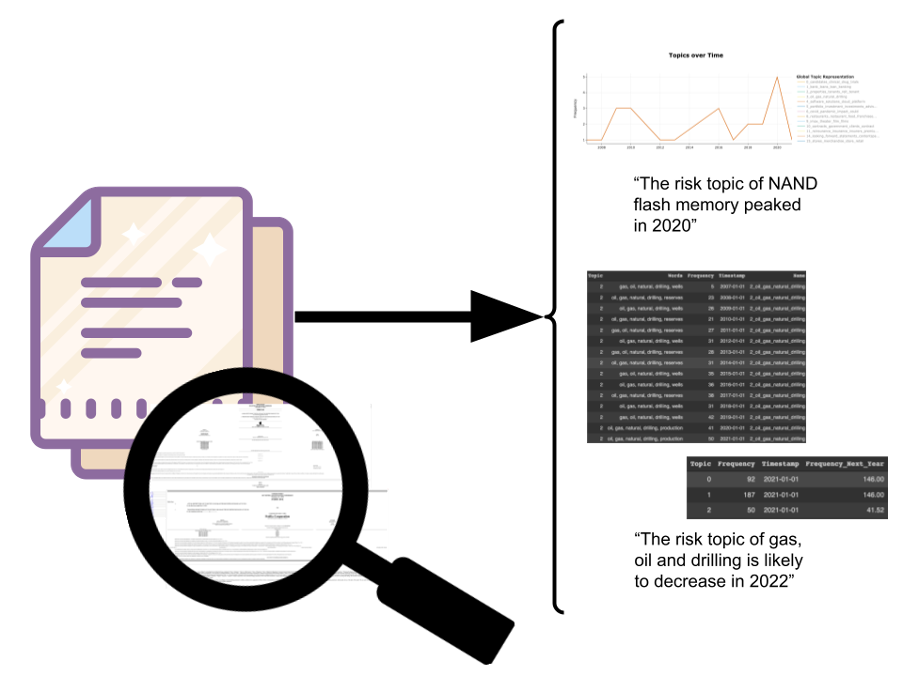
\includegraphics{images/abstract/Aim_image.png}
\caption{A visualisation of what the aim of the project is}
\end{figure}

\section{Objective}
\begin{itemize}
  \item Extract annual reports from SEC-EDGAR
  \item Extract section Item 1A. Risk Factors from the HTML version of the report
  \item Extract topics from the corpora using BERTopic
  \item Forecast evolution of topic importance and analyse the results
\end{itemize}

\section{Outcomes}
This project has resulted in:
\begin{itemize}
  \item A topic modelling pipeline to process a large corpus of unstructured
text
  \item A BERTopic implementation to track topics throughout a timeframe
  \item A classifier model predicts if a topic will increase in ‘importance.’
  \item A regression model to forecast the importance of a topic next year
  \item A time-series forecasting prototype model for the importance of a topic
\end{itemize}

\chapter{Background}

\section{Financial reporting}
SEC stands for U.S. Securities and Exchange Commission. “The primary purpose of the SEC is to enforce the law against market man." \cite{wiki:sec}. This governmental body provides the most extensive database for financial documents in the U.S. All information reported by a company is stored as a submission and later extracted into XBRL data. They are available via RESTful APIs on data.sec.gov \cite{sec-api-docs}, offering JSON formatted data or directly on a submission index page as HTML and XML.

\begin{figure}[h]
    \centering
    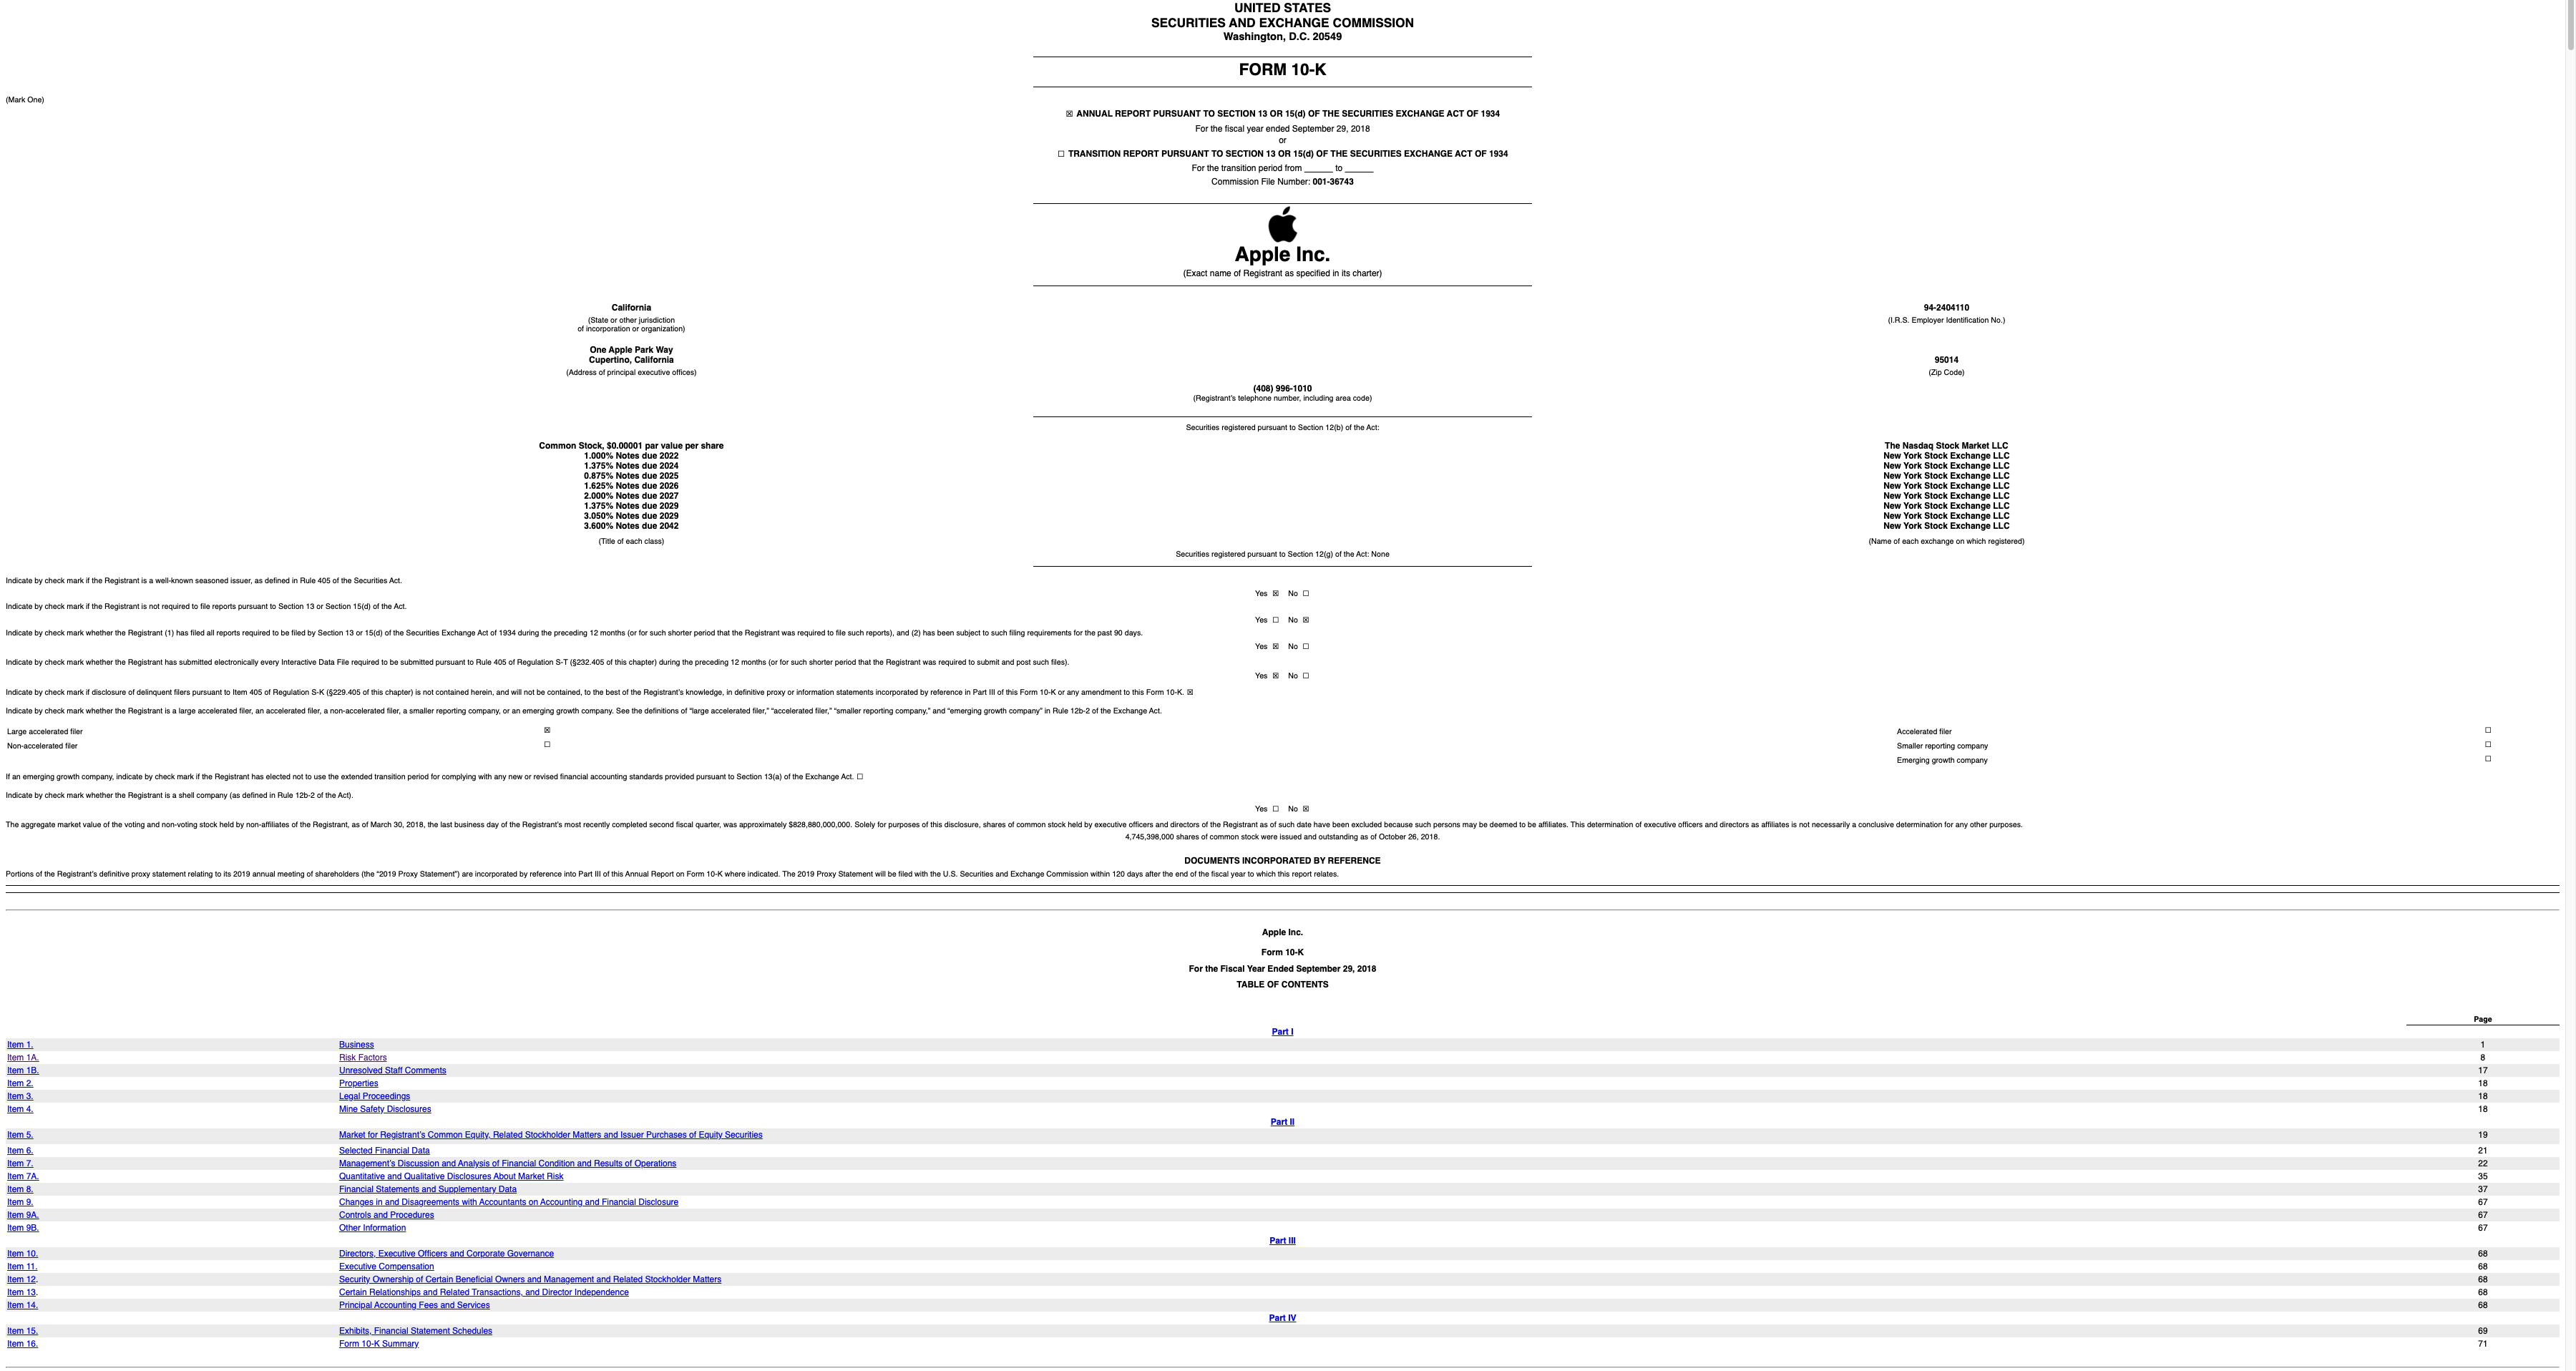
\includegraphics[scale=0.1]{images/Example Annual Report.png}
    \caption{An example of digitalised report \cite{digitalised-report-example}}
\end{figure}


The companies are encouraged to use the Electronic Data Gathering, Analysis, and Retrieval system \cite{edgar-search} to query this data. The latest version of this tool was launched in 2001 according to \cite{edgar-search} and allowed querying over the entire database. Even though this does not force foreign companies to report, it still includes a large share of the biggest companies in the world, 126 from \cite{fortune-500-2021}.

\subsection{10K Forms}

A Form 10-K is an annual report submitted to the SEC that gives an exhaustive overview of a company's economic performance. "The 10-K includes company history, organisational structure, executive compensation, equity, subsidiaries, and audited financial statements, among other information"\cite{wiki:10k}. According to the latest regulation, they are submitted around the same period according to \cite{10k-general-rules}, making the specific submission date irrelevant for further processing. Companies are separated into multiple subcategories based on several criteria. One of those splits them into "smaller reporting" or" large accelerate" filers. Previously to 2009, the first category had the option to submit a different report. They represent a complete data source in unstructured textual form for the company. Even from a structural and aesthetic point of view, there are certain liberties that each company takes. There are multiple guides to understand the information disclosed, one directly from SEC and several others. 

\subsection{Item 1A – Risk Factors}

In this section, "the company lays anything that could go wrong, likely external effects, possible future failures to meet obligations, and other risks disclosed to warn investors and potential investors adequately" \cite{wiki:10k}. Typically, they are listed in order of their importance. Risks can be considered \textit{general risks}(for the entire economy) and \textit{specific risks}(that apply only to the company's domain, geographic region, unique to the company). Smaller reporting companies are excepted to do so. However, some companies still disclose them voluntarily or offer an overview for their investors. There are no clear guidelines regarding the language used to disclose risks: the same risk can be described in different terms in two other places.
Throughout time this section suffered multiple legislative modifications. One main changes affected the dataset:

In 2020 they allowed the use of hyperlinks to avoid duplicates. Moreover, they enforced that if the section surpasses 15 pages, a summary with references should be submitted instead of the complete risk analysis.(source: \cite{modernisation-ruling})

\section{NLP}
NLP(Natural Language Processing) refers to the branch of Computer Science, particularly artificial learning, that allows programs to process, understand and derive meaning from human languages in different forms. It has its roots in the field of linguistics and artificial intelligence. However, as the digital world started expanding, there is a need to capture this facet of our reality, analyse it and reproduce it digitally. Natural language processing has a wide range of applications in business. This domain combines data science, software engineering, and linguistic modelling to achieve marvellous commodities such as spelling and grammar auto-correction, text support, speech recognition, text to speech translation and many others. The amount of data in an unstructured form that is being generated is increasing, and there is no sign of the trend slowing down.

\begin{figure}[h]
    \centering
    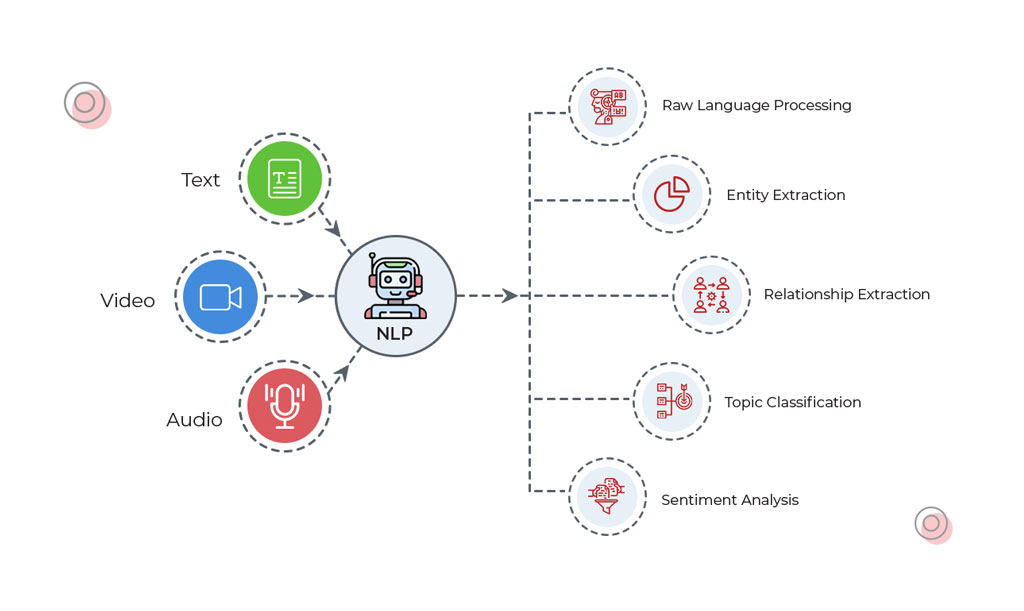
\includegraphics[scale=0.5]{images/abstract/NLP_Processing.jpg}
    \caption{Representation of Natural Language Processing applications}
\end{figure}

\section{Sentence Embeddings}
One of the main components that allow this pipeline to work is sentence embeddings. For any algorithm, it is hard to interpret and process string values. That is why, to process sentences, we need a mapping for them into vectors. Those mappings are obtained through a collective set of techniques categorised as sentence embeddings. The main goal is to capture a range of semantic relationships between sentences, the most important in this case being similarity. Compared to contextualised word embedding, which embeds every word from a sentence based on the context, starting from a traditional word embedding view, a sentence embedding creates one representation for the entire sentence. A contextualised word embedding represents a word in a context, whereas a sentence encoding represents a whole sentence.

\section{BERT}
BERT stands for Bidirectional Encoder Representation from transformers. It is the architecture of state of the art for Masked Language Modeling and Next Sentence Prediction, two significant NLP challenges. It was developed by Google and appeared in \cite{DBLP:journals/corr/abs-1810-04805}. It is based on the transformer architecture proposed by \cite{DBLP:journals/corr/VaswaniSPUJGKP17}. When processing text, one of the main bottlenecks that appeared since the beginning of the development of NLP was the direction in which we are inputting sequentially. Transformers allowed us to input it non-directionally. BERT takes a sequence of tokens generated from a text as an input, usually a sentence. These tokens are embedded on three levels, word, segment and positional. It utilises popular word embeddings on a word level, adding a [CLS] token to all the instances where the input word is present and a [SEP] token to keep track of where the sentences end. Then, at a segment level, a marker is set to indicate a mapping for each sentence. The last level is positional, saving the actual position of each token in a sentence. The representation formed is fed into a deep learning architecture. For example, BERT-Large has 24-layer, 1024-hidden-nodes, 16-attention-heads and 340M parameters. This output is also a vector that perfectly mirrors the original tokens positional structure.

\begin{figure}[h]
    \centering
    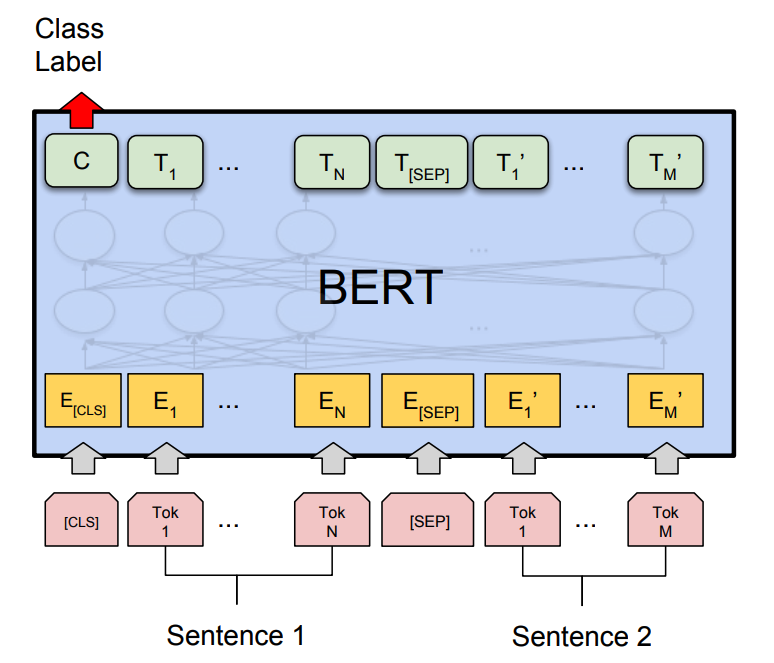
\includegraphics[scale=0.5]{images/abstract/bert.png}
    \caption{A visualisation of the architecture behind BERT}
\end{figure}

\section{Topic Modelling}
Topic modelling is a subdomain of NLP that studies methods to extract the topic described in a sequence of text. It is a valuable branch of this area, especially when the processing target is a large dataset. The goal is to unravel hidden representations or trends. The definition of a topic is a loose term here. Intuitively, topic refers to the dominant cluster from a text segment, representing a common meaning for all those words. When looking at a report, we can quickly visually observe certain words and key terms to understand the overarching motive of that text. Human brains emit a guess regarding the activity in that a company is involved.
Moreover, we can argue that multiple topics can be underlined in a single document by utilising this definition. Several probabilistic models help discover the probabilistic distribution of topics in extensive collections of unstructured text. It is widely used in text mining, sentiment analysis or summarization algorithms.

\begin{figure}[h]
    \centering
    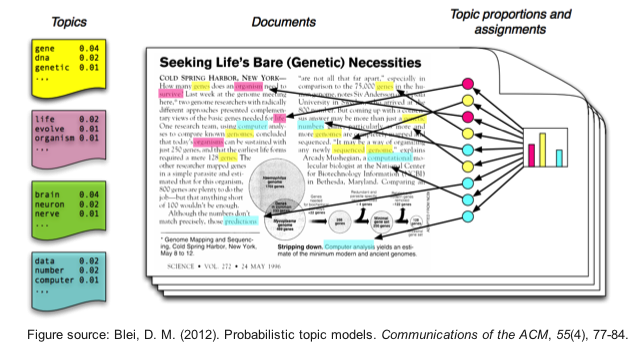
\includegraphics[scale=0.5]{images/abstract/Topic Modelling Example.png}
    \caption{A visualisation of Topic Modelling}
\end{figure}

\section{Dynamic Topic Modelling}

Dynamic topic modelling (DTM) is a collection of techniques to analyse the evolution of topics over time. These methods allow understanding how a topic is represented differently. There are multiple ways two different companies talk about the same topics. Moreover, the same concern for a company can take different facets throughout the time, reflected in different terminology supporting the same topic. These issues result in an issue for tracking the evolution.

\begin{figure}[h]
    \centering
    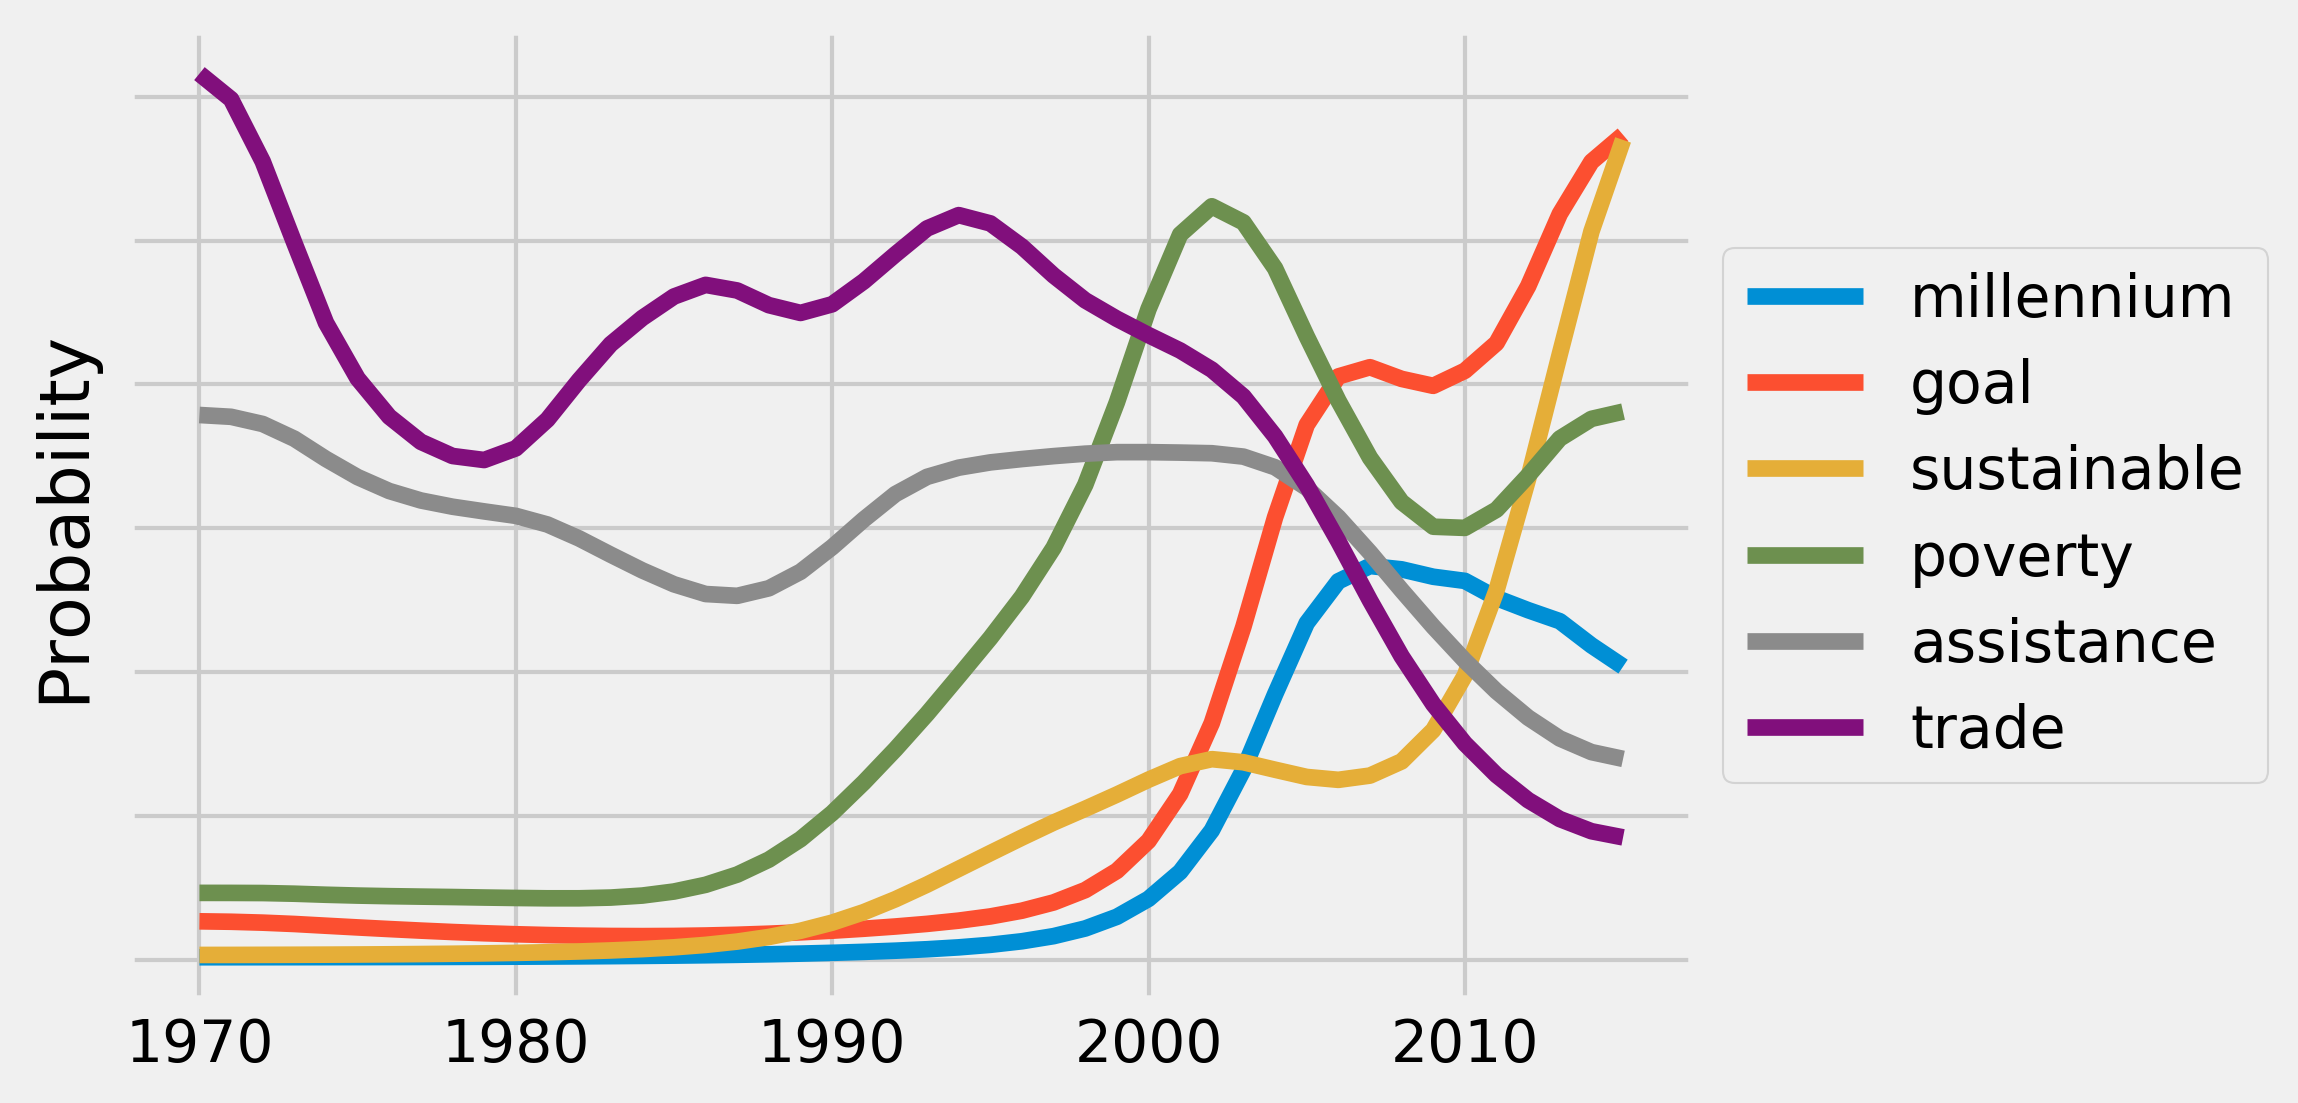
\includegraphics[scale=0.17]{images/abstract/DTM example.png}
    \caption{An example from \cite{dtm-example}}
\end{figure}

\section{BERTopic}

\begin{figure}[h]
    \centering
    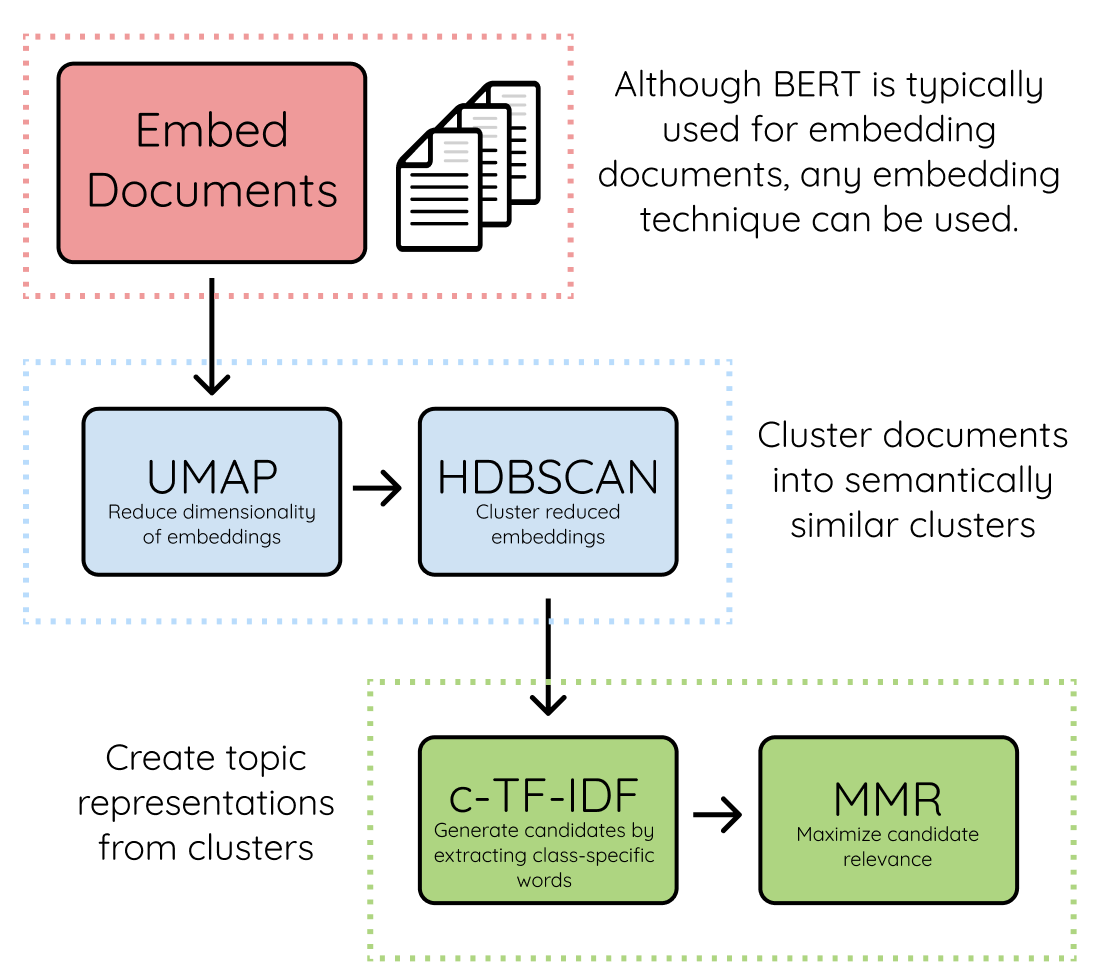
\includegraphics[scale=0.3]{images/abstract/BERTopic pipeline.png}
    \caption{A visualisation of the pipeline from \cite{grootendorst2020bertopic}}
\end{figure}

BERTopic is a state-of-the-art NLP pipeline created by \cite{grootendorst2020bertopic}. It can be used with multiple transformers and c-TF-IDF to form dense clusters allowing for easily interpretable topics whilst keeping essential words in the topic descriptions. It utilises BERT pre-trained models for embedding the documents into high dimensional representations. From that step, it uses UMAP \cite{umap} to reduce the dimensionality of the embeddings. The previous step facilitates the clustering performed afterwards by HDBSCAN \cite{hdbscan}. It is a popular high dimensional clustering algorithm for high dimensional data. In the last step, the paper outlines how it utilises c-TF-IDF in this context. It takes the basic principle behind TF-IDF but replaces documents with clusters. The Term frequency is defined as the number of times a term appears in a cluster(class). The document frequency is defined as the number of times a word relates to a topic is referenced across the entire dataset.

\section{MACD}

\begin{figure}[h]
    \centering
    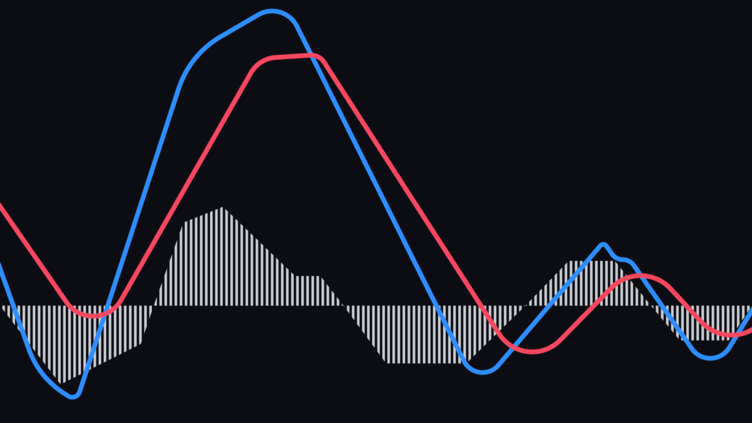
\includegraphics[scale=0.55]{images/abstract/MACD Bin.png}
    \caption{MACD lines}
\end{figure}

MACD stands for moving average convergence divergence (\cite{wiki:macd}). It appeared in late 1970. It was used as a trading indicator. It embodies indicators for both current production and performance but also desired results. This characteristic is what made it appealing to the trading world. From a mathematical point of view, it represents three different time series from historical data(in the case of this project, the importance of a topic). It approximates the acceleration of the significance throughout the timeframe at each timestamp. It depends on three parameters, dictating the time windows used for calculations. The most frequent one is (12, 26, 9), on a daily time series. However, the version used in this project is an (8,4,2) configuration, being annual. The three signal lines represent MACD, an average(also called Signal in the implementation) and Histogram, the difference between the last two signals. MACD line is represented by the difference between a long rolling average over the previous 8 timestamps and a short rolling average over the previous 4. The average Signal value is generated by averaging MACD over the last 2 timestamps.
This approximation is widely used in multiple applications, even though it can lag between the trend modelled and the actual timing of the evolution.

\section{Related Research}
The initial ideas started from the references offered in the project description. \cite{lafferty_blei_2009} introduces the idea of topic modelling as an option to analyse and describe a large dataset. They used a hierarchical Bayesian analysis, \cite{ghosh2006introduction}, and Latent Dirichlet Allocation(LDA, \cite{blei2003latent}). They describe Dynamic Topic Modelling(DTM) and Correlation Topic Modelling(CTM) as extensions to LDA. The state-of-the-art approaches running today are based on the same methods presented there. The disadvantage of using LDA is the number of topics, and the actual representation, which needs to be fixed in advance.
\cite{Blei2010ProbabilisticTM} introduces a new method called dynamic Hierarchical Dirichlet processes. This procedure allows for the concept of evolving topics over a timeframe. It fits the documents over the terms at a timestamp \textit{t}, rather than using terms from the entire document collection. Another downside of LDA is present here: the basic unit of a \textit{topic} is still considered a \textit{word}, either called \textit{keyword} or \textit{candidate term}.
Flexiterm, \cite{Spasi2013FlexiTermAF}, presented a new point of view to approach the task. It is based on the C-value, \cite{Frantzi2000AutomaticRO}, but offers more flexibility. However, the definition used in this research work for a \textit{topic}, as a bag of words approximately matching the same term, is vastly different from the approach needed in the particular case of this pipeline, where words need to represent a unified meaning.

Looking back at other projects that tackled the same challenge, Dhruv \cite{dhruv}  presented another methodology to analyse an older but similar dataset. The pipeline proposed by his work focuses on keyword extraction, following the paths set by LDA. After that, it uses a pre-trained FINBERT (\cite{DBLP:journals/corr/abs-1908-10063}) model, fine-tuned BERT(\cite{DBLP:journals/corr/abs-1810-04805}) variation for financial documents, for sentiment analysis on the sentences from the reports. The topic modelling part was limited to implementing Top2Vec(\cite{top2vec}) and analysing the representations obtained. However, that was not the aim of the project. That was to detect emerging topics. Moreover, the dataset from that article is a small subsample. The method of acquiring that level of accuracy during data mining is unclear.
Bursty terms in computer science research by \cite{Tattershall2019DetectingBT} presented a novel way to track and predict the evolution of specific keywords in a corpus. It utilises a heavyweight pre-processing technique for text mining before creating a vocabulary and employing popular trading indicators as features for the topics. It utilises a \textit{RandomForestClassifier} from sklearn (\cite{scikit-learn}) to determine which \textit{topics}, viewed as a cluster of \textit{n-grams} with similar embeddings, will burst in the future. While the methodology operated is advanced and fits the aims of this project, I faced a problem during the implementation phase, the limited range of the dataset. In that approach, the data range was between 1988 and 2017, while mine was limited to only 14 years. The limitation of the dataset is related to the digital format from which the risk factor sections are extracted, which started a consistent run from 2007 to 2021.
One takeaway from that article was the MACD (\cite{wang2018predicting}). It was utilised as a feature for the classifier and regression models.
Finally, the research led to the BERTopic library(\cite{grootendorst2020bertopic}). The main strengths of BERTopic, its state-of-the-art performance while being flexible for a plethora of pre-processing options and embedding models, were utilised in the following pipeline.
Moreover, the modularity of this process is being tested with intermediary results and fine-tuning at every level available. The performance claims in topic diversity and topic cohesion are not reevaluated here, as this is not part of the project's aim. The results regarding wall time presented in the paper are too broad from my perspective. The pre-trained models used there are not being declared how they are used. As the following chapters will see entail, the library used to perform the actual embedding, alongside the pre-processing procedure allocated, can drastically impact the results.

\chapter{Implementation}

\section{Requirements}
There are specific requirements that the implementation must fulfil to be considered practical:
\begin{itemize}
  \item Batch based, continuous data extraction
  \item Reliable and reproducible risk section extraction
  \item Scalable storing and indexing capabilities for the entire pre-processing pipeline for textual data
  \item Modular implementation of BERTopic
  \item A machine learning model to utilise the data outputted by topic modelling
\end{itemize}
\newpage

\section{Configurations used}

\begin{table}[h]
  \caption{Configurations used}
  \label{tab:freq}
  \begin{tabularx}{\textwidth}{|X|X|X|X|X|}
    \toprule
    {Configuration name}&{CPU}&{RAM}&{GPU}&{OS}\\
    \midrule
    A & AMD Ryzen 5 4600h & 32GB & NVIDIA GeForce® GTX 1650 4GB GDDR6 & Windows 11\\ \hline
    B & AMD Ryzen 5 4600h & 32GB & NVIDIA GeForce® GTX 1650 4GB GDDR6 & openSUSE Tumbleweed\\ \hline
    C & Apple M1 & 16GB &  & macOS Monterey 12.3\\ \hline
    D & 1.7GHz quad-core Intel Core i7, Turbo Boost up to 4.5GHz & 16GB & Intel UHD Graphics 128MB of eDRAM & macOS BigSur 11.6.5\\ \hline
    E (Google Colab Pro+) & 2 x Intel Xeon @ 2.199GHz & 52GB & NVIDIA K80 & Ubuntu 18.04.5 LTS\\ 
  \bottomrule
\end{tabularx}
\end{table}

\begin{figure}[h]
    \centering
    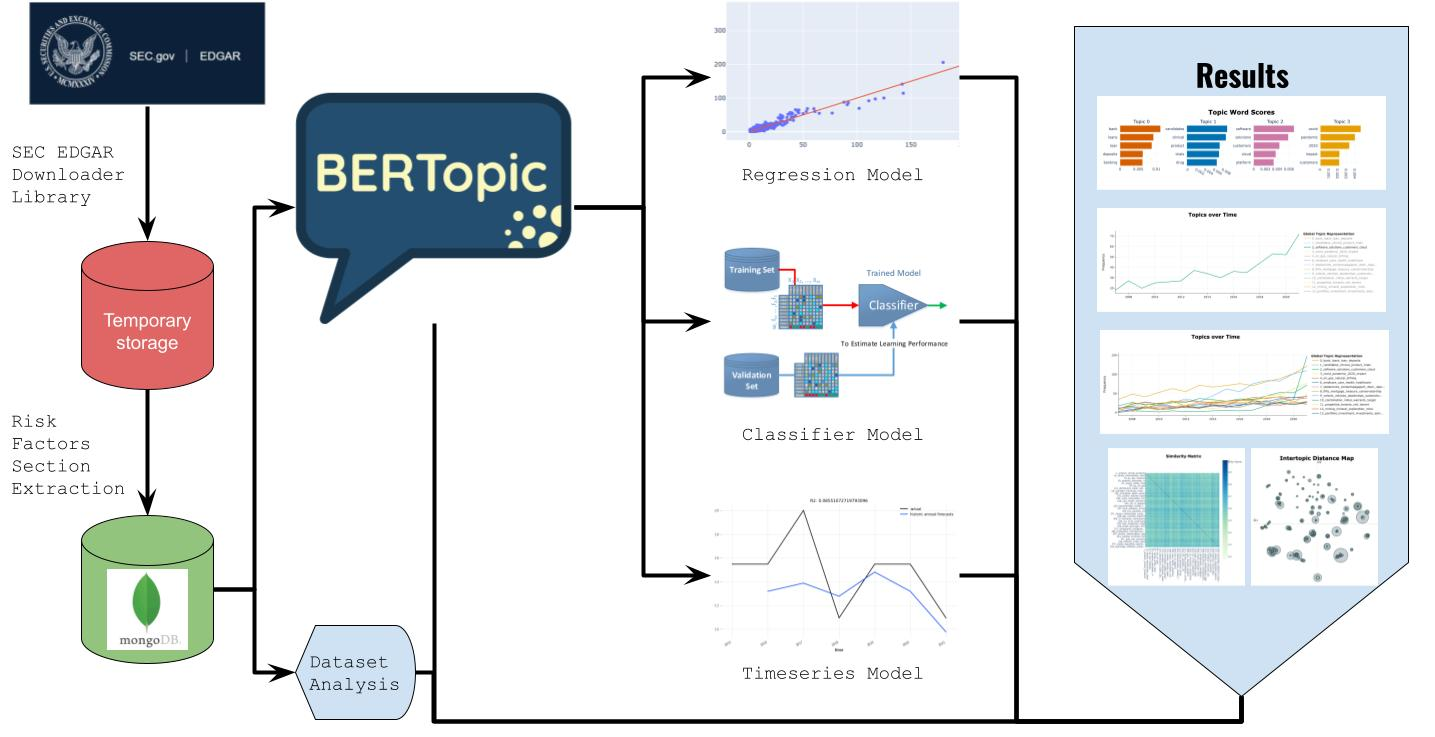
\includegraphics[scale=0.25]{images/Thesis pipeline.jpg}
    \caption{A visualisation of the pipeline proposed by this project}
\end{figure}

\section{Data pre-processing}

\subsection{Data Mining}

I initially tried to manually build a data-mining script utilising SEC EDGAR's API to obtain the data. This approach was going through the submission history for each quarter, filtering all 10K submissions, altering the original URL (which most of the time would point to the index page of the submission), sending a POST request and retrieving one specific file back. This approach failed due to being slow (Many documents would be submitted in a quarter, which led to prolonged processing times to filter 10K reports. This issue becomes inadequate due to the API's number of requests per second restriction of 10. An example of how long one quarter would take (\ref{appendix:1}.1)
After that, I found the sec-edgar-downloader library \cite{sec-edgar-downloader}. It is a company fillings downloader that utilises a stock ticker or a Central Index Key (CIK). Even though the download files would include the complete submission index, it solved the need to filter 10K reports for each company based on quarter. That leads to the final approach for the data-gathering phase. Using the CIK mapping file by SEC-EDGAR \cite{sec-company-tickers}, I looped through all the registered companies and extracted all the 10K reports available. They would come in .html format. I used BeautifulSoup,\cite{bs4} library to parse the files. Initially, I thought the entire dataset could fit in a master tabular file. However, as the data extraction method was working, I noticed that the size of this dataset would be unmaintainable using this idea.(\ref{appendix:3}.3). The next and final approach for storing the documents was using a local MongoDB instance. MongoDB is a NoSQL, document-oriented database with high scalability and speed focus \cite{mongodb}. Moreover, I decided that there was no need to store all the reports and additional files, so I created an ETL process \cite{etl} to handle the data-gathering phase:

\begin{figure}[h]
    \centering
    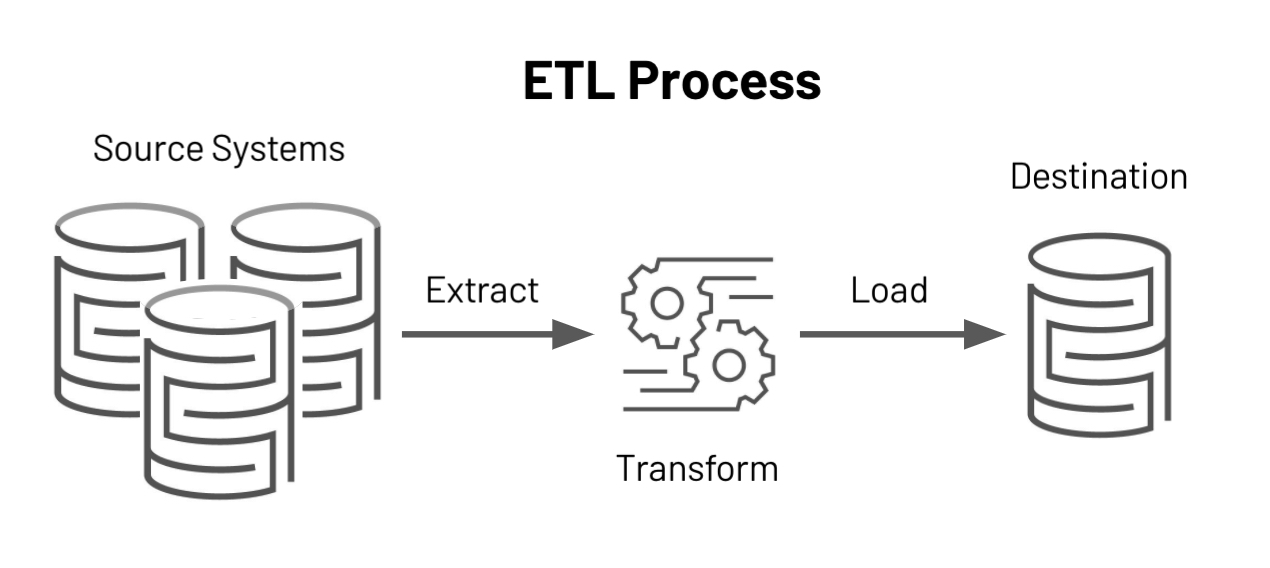
\includegraphics[scale=0.3]{images/abstract/ETL-Process.jpeg}
    \caption{A representation of ETL from \cite{etl}}
\end{figure}

\begin{itemize}
  \item Extract: using the \textit{sec-edgar-download library}, it would download the entire 10K submission, from which I would only keep the \textit{filling-details.html}.
  \item Transform: The document would be parsed using BeautifulSoup. It would then be processed by the risk factors extraction method to produce multiple fragments.
  \item Load: Each fragment would be loaded into a collection from MongoDB as a document. The fields stored in a document are:
      \begin{itemize}
          \item Ticker: \textit{str} to keep track of which company this fragment belongs to
          \item Year: the year for which the statement was reported
          \item Start\_index: the index at which the fragment started in the original document
          \item End\_index: the index at which the fragment ended in the original document
          \item Size: the size of the risk factors in characters
          \item Text: the parsed text extracted from the original document
      \end{itemize}
\end{itemize}

For this entire process, there are three parameters to fine-tune its performance: 
\begin{itemize}
          \item Upl\_text: int - the maximum multiplication factor between index \textit{1A} and index \textit{1B} positions. For example, suppose the keyword \textit{1A} appears at position 3240 and upl\_text is set to 10. Any \textit{1B} occurrence at a position greater than 32400 will be considered too far away to form a Risk Section.
          \item lrts: int - Lower boundary from which fragments become relevant data. For example, if the algorithm extracts a 100 character fragment of text and lrts=200, that fragment will be discarded.
          \item targeted\_document: either \textit{latest} or \textit{legacy} .\textit{latest} will use the XHTML file, a web-ready version, which retains the information better after parsing. \textit{legacy} - is a text-based version, which keeps the document structure and readability better.
\end{itemize}
This entire stage is implemented in \textit{data\_gathering.ipynb}. 

\subsection{Risk factors section extraction}

One of the main challenges was regarding the data gathering process. Extracting the risk factors section raised multiple problems that appear after parsing the documents:
\begin{itemize}
          \item The XHTML formatting used differs for each company. For example, some companies started the section immediately after the heading, without any separator tag, often creating erroneous tokens, such as \textit{ Item 1.A:Risk FactorsTh} (\ref{appendix:4}.4). This different formatting also confused the parsing library, which sometimes parses documents as HTML, sometimes as XML, and sometimes crashes, reporting encoding errors. The latter was fixed soon after by enforcing the standard UTF-8.
          \item The exact section can be referenced throughout the entire report. That would lead to different fragments of text being categorised as part of the risk factors section. Any structural element would not delimit those fragments. (\ref{appendix:5}.5)
          \item The first occurrence of the terms used to extract the information would always appear in the table of contents. If the parsed results were not perfectly separating the tokens, it might lead to the entire table of contents being included before the actual risk factors or only a short paragraph from it(\ref{appendix:6}.6)
\end{itemize}

To tackle this issue, I employed a keyword-based index extraction. I tried looking for a better technique. However, due to the large data gathering undertaking, none of the more advanced techniques(\cite{SOUILI2015635},  \cite{clarity-nlp}) would justify the time investment needed to reproduce peak performance. This approach was inspired by the previous work Dhruv completed on the same project\cite{dhruv}. The implementation can be seen here (\ref{appendix:2}.2).
 
Using a regex, I would get the index of every \textit{Item 1A} and \textit{Item  1B} appearance from the document into two lists. Afterwards, a while loop will run until one of those two lists runs out, checking if \textit{index\_of\_item\_1a} is smaller than \textit{index\_of\_item\_1b}. In a 10K report, the Risk Factors section should always come before item 1B. An insignificant amount of reports lacked section 1B and led to erroneous extraction. To deal with this edge case, the\textit{ upl\_text} parameter can be set.
At each iteration, the \textit{index\_of\_item\_1a} will be multiplied by \textit{upl\_text }and checked if \textit{index\_of\_item\_1b} is still larger than it. This check ensures that the character distance between the Item 1A and Item 1B is not too big, pointing clearly to a wrong combination of indexes and a noisy text fragment. In this case, a noise fragment is defined as one which embodies anything else besides the risk factors section. After getting a valid combination of indexes, the fragment of text between those indexes would be extracted and stored in the database as a separate document, alongside the metadata aforementioned.
 In addition to all of that, there is also a simple mechanism to log the data gathering process. At each iteration of a ticker from the complete list, a filter removes all documents with a character length smaller than the \textit{lrts} parameter. This procedure ensures that only big enough fragments are stored to represent the risk factor section.
To determine the best performance, both parameters were thoroughly tested using the same set of companies''MSF'',''AAP'',''GOO'',''AMZ'',''TSL'').(\ref{appendix:7}.7) 

For \textit{lrts}, the default value(50) was selected based on the shortest fragment extracted from the first 100 companies extracted. I decided to keep it that way to remove any random short string and allow any other quicker extraction, even though that would include other references. They would be shortened and sometimes pre-processed later pipeline steps. Moreover, references would also link certain risk factors to essential keywords in certain edge cases.
An entire run of the data gathering process took 184 hours, 54 minutes, and 13 seconds using configuration B.

\clearpage

\subsection{Dataset Analysis}

\begin{figure}[h]
    \centering
    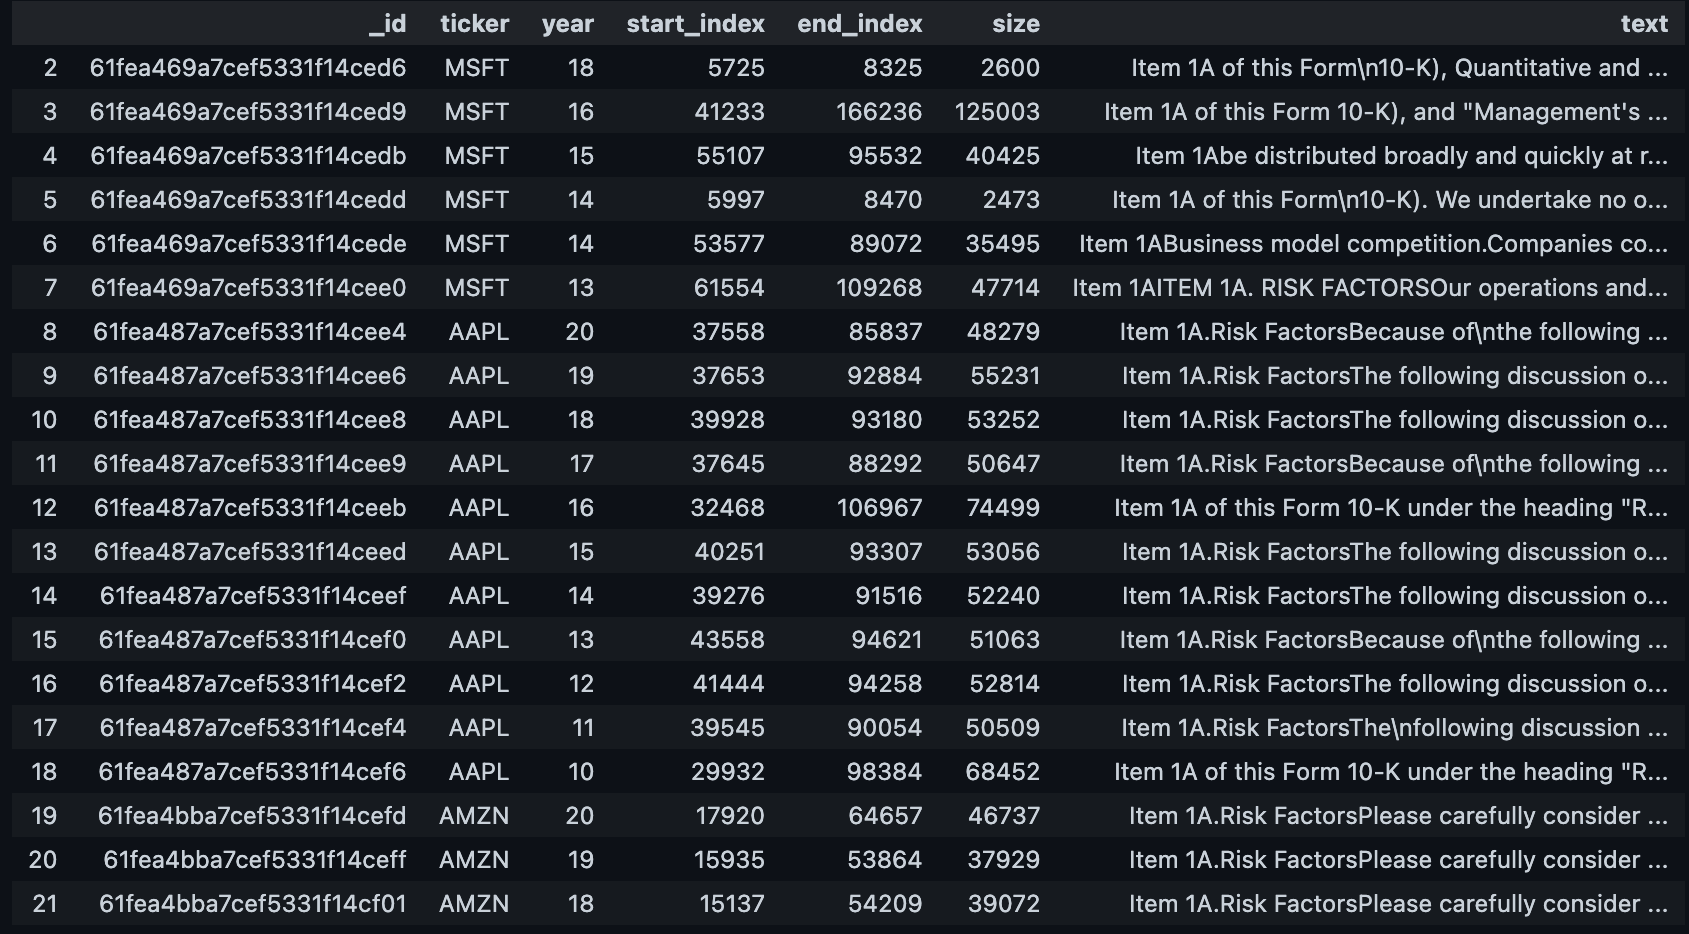
\includegraphics[scale=0.4]{dataset_analysis/extract_dataset.png}
    \caption{Extract from the complete dataset}
\end{figure}

The next step was the analysis of the dataset. The total number of fragments extracted, each as a document in the MongoDB collection, was 29457.

\begin{figure}[h]
    \centering
    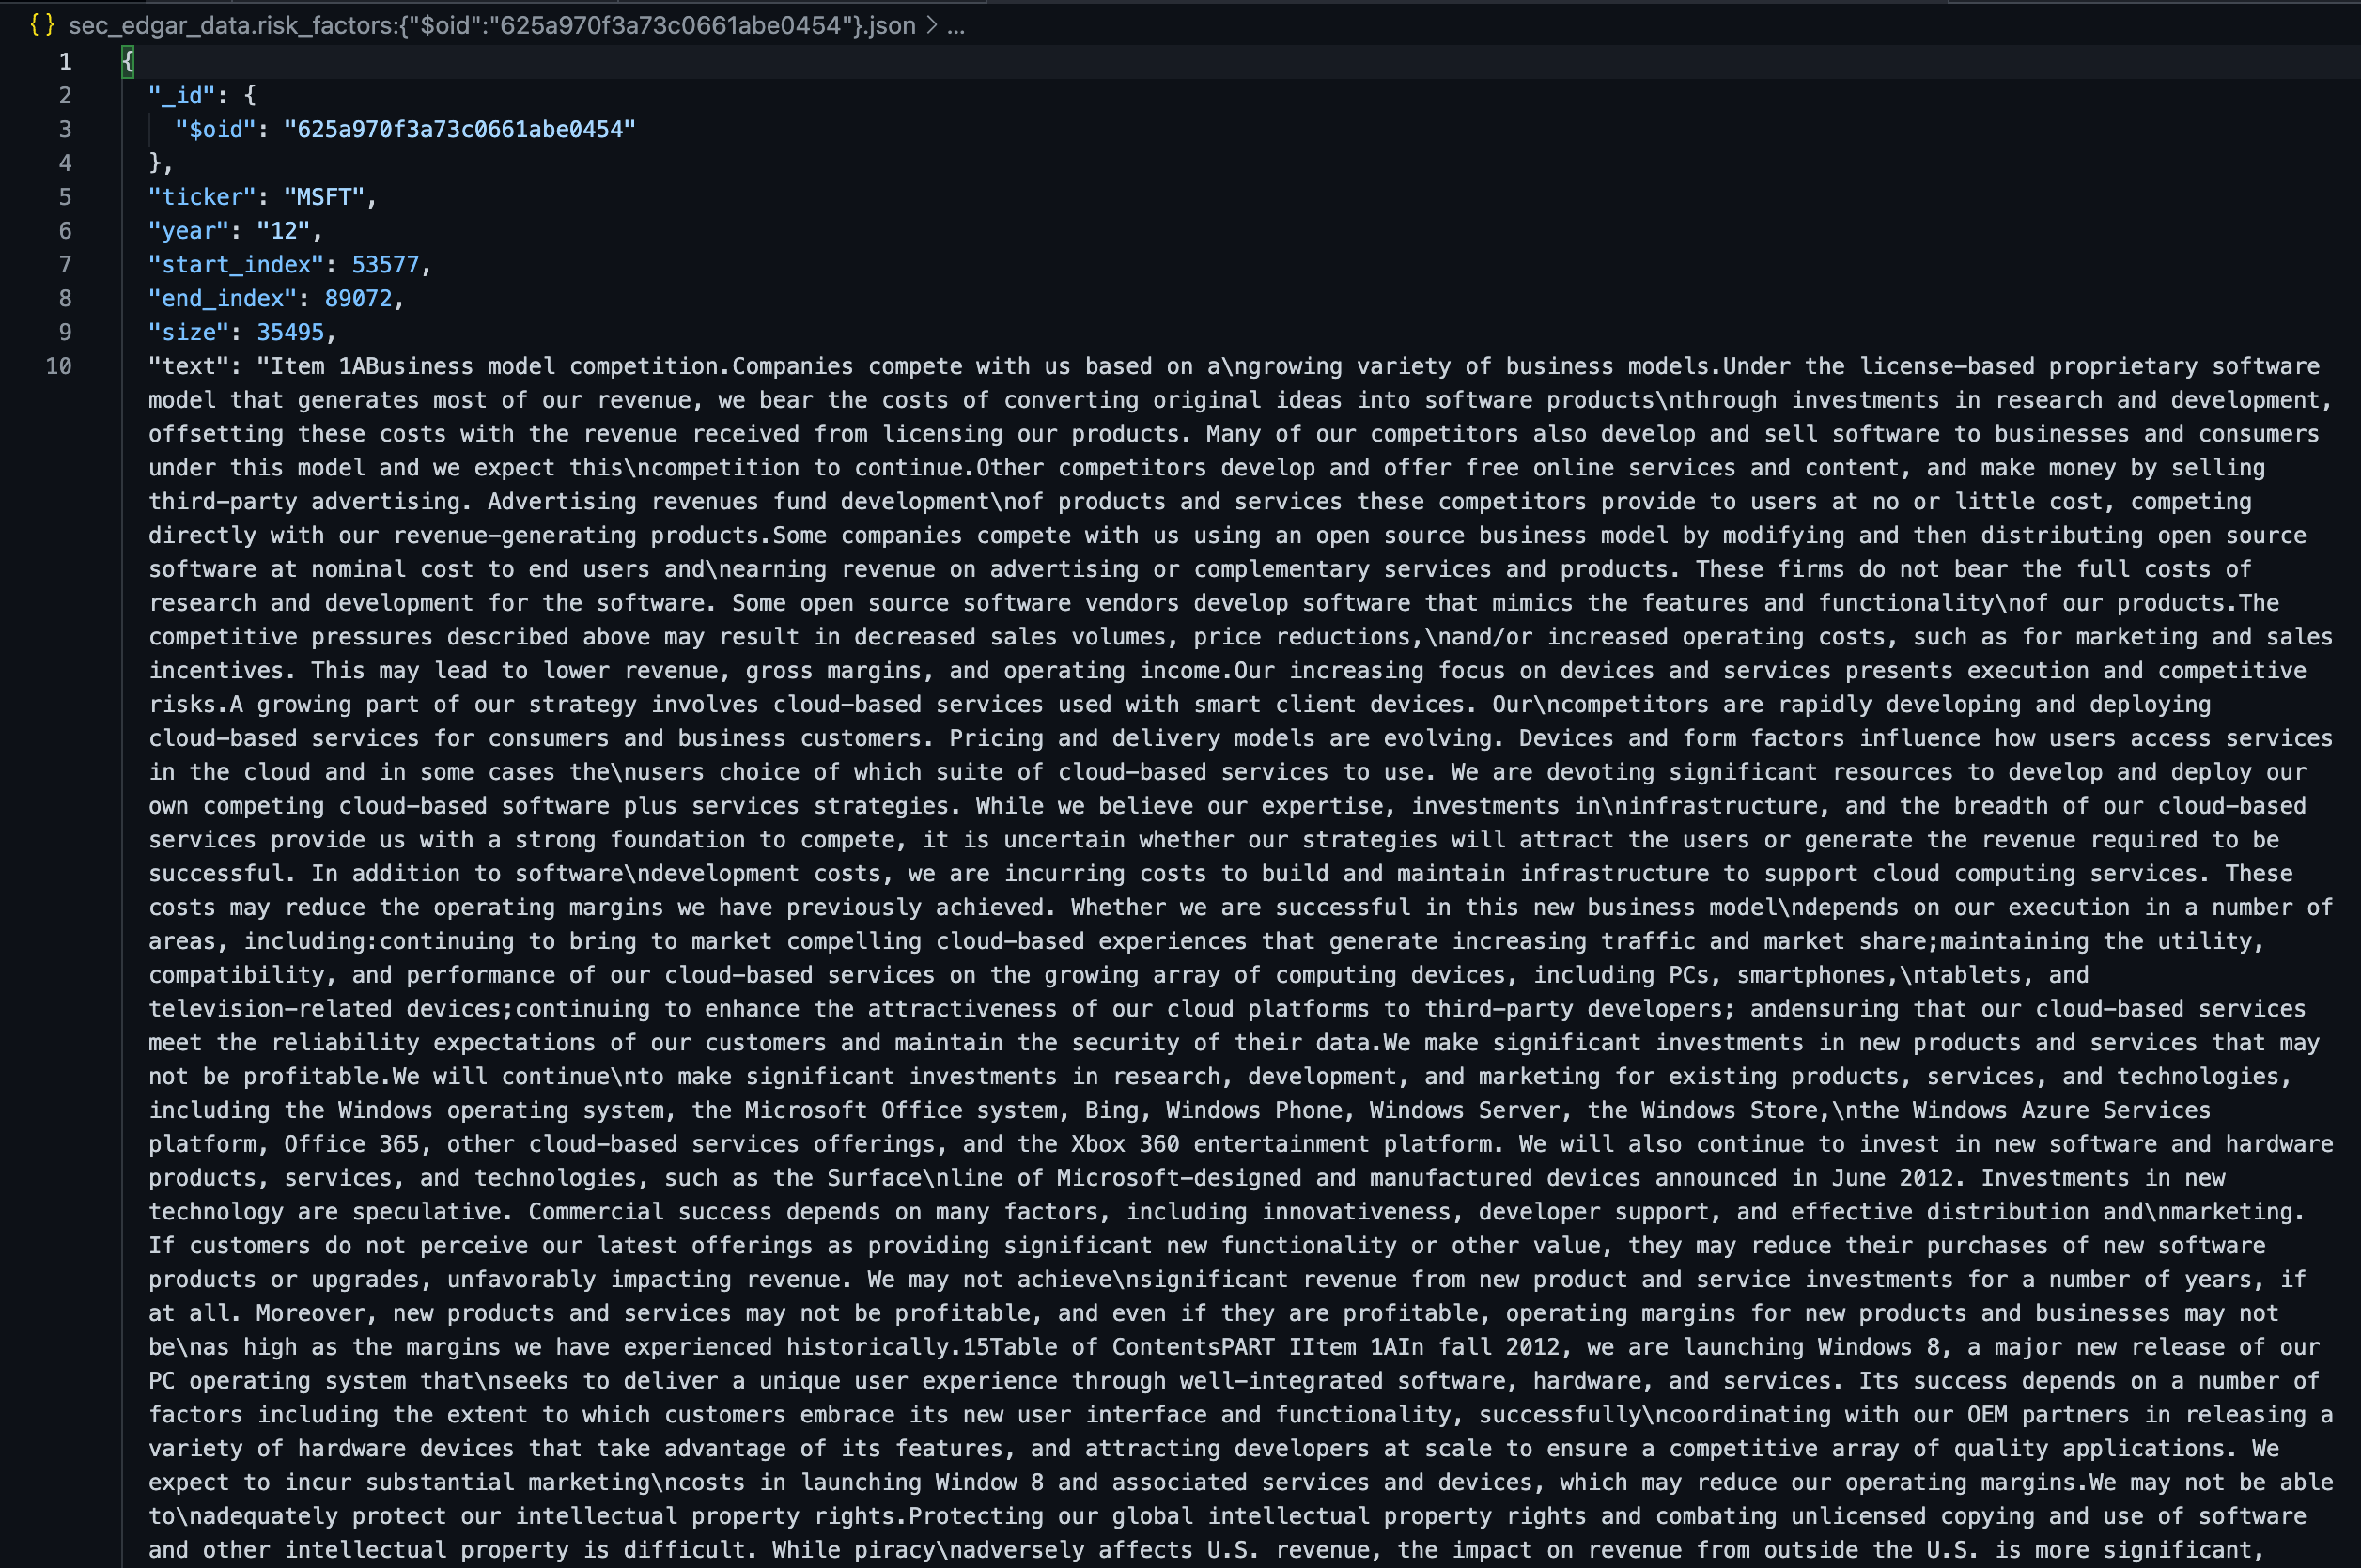
\includegraphics[scale=0.2]{dataset_analysis/example_fragment.png}
    \caption{One extracted fragment}
\end{figure}

There are multiple observations to be made from here:
\begin{itemize}
    \item ‘\textbackslash n’ character needs to be removed.
    \item There is no clear separation between sections.
    \item The parsed document retains the text in good condition, with a few instances where a wrong token can be deducted.
\end{itemize}

To support several decisions for the later stages of the pipeline, I started by performing an exploratory data analysis.
\begin{figure}[h]
    \centering
    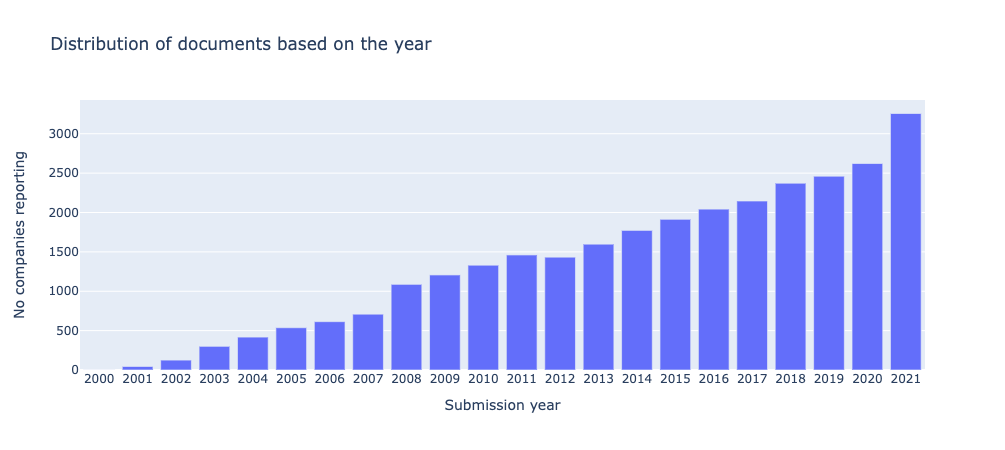
\includegraphics[scale=0.4]{dataset_analysis/Yearly Distribution document.png}
    \caption{Yearly distribution of the fragments extracted}
\end{figure}

This distribution is justified by the number of documents made available through the new EDGAR platform “The new EDGAR advanced search gives you access to the full text of electronic filings since 2001” (\cite{edgar-search}). The changes started in 2001, and it has been increasing ever since.

\newpage

\begin{figure}[h]
    \centering
    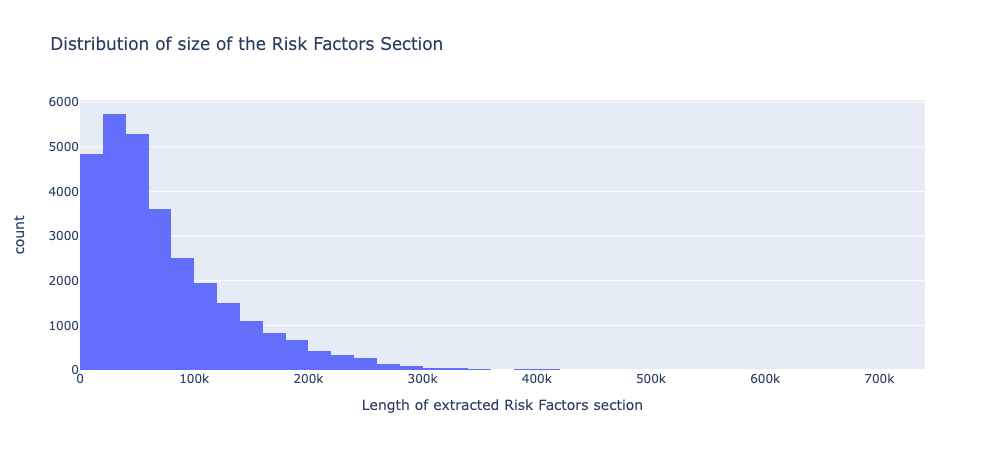
\includegraphics[scale=0.5]{dataset_analysis/Distribution of size.png}
    \caption{Distribution of the fragments extracted based on their size in characters}
\end{figure}

\begin{itemize}
          \item The longest fragment extracted is 740K characters long (after manual inspection, it turned out to be an erroneous one)
          \item The 90th percentile is 159855, and the 99th percentile is 277633. I wanted to use all the data under the 99th percentile for the rest of the pipeline. However, due to computing limitations, I had to set the upper limit for the size of the fragments, 220000. Moreover, later in the research phase, I discovered that even the 90th percentile would lead to good results for the later processing done in the pipeline.
          \item  The most populated size bin is between 20K and 40K, with 5745 documents.
\end{itemize}

\begin{figure}[h]
    \centering
    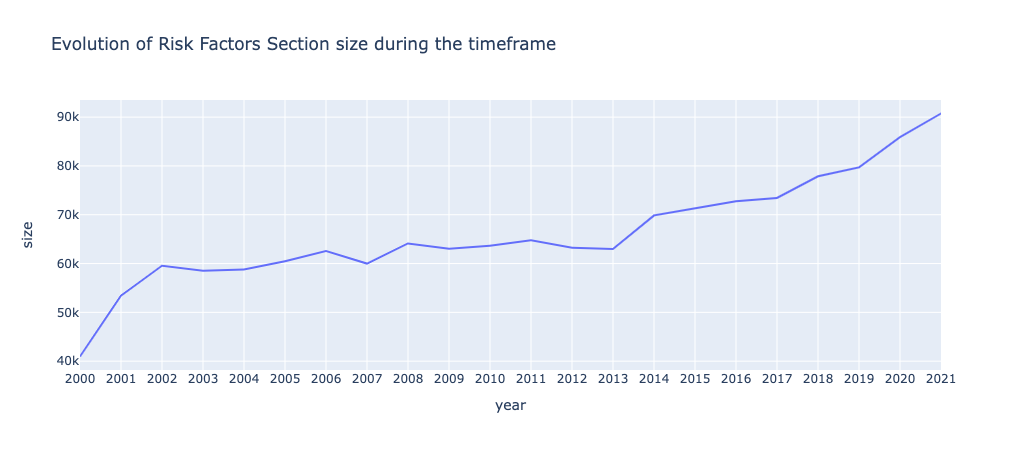
\includegraphics[scale=0.5]{dataset_analysis/Evolution of size .png}
    \caption{Evolution of extracted fragments size throughout the years}
\end{figure}

The latest part of the analysis was to check if there was a trend in the size of the fragments extracted through time. There are two significant increases from 2000 to 2002, explained by the introduction of the new system and more documents being filed there, and on more from 2013 till the present day. One more important observation is that the dataset includes smaller reporting companies due to the laborious undertaking required to remove them, thanks to a lack of mapping between CIK and the type of company. They will be clustered together into a topic and released later in the pipeline.

\subsection{Pre-processing}

During the development of this pipeline, I researched multiple approaches to pre-processing textual data. According to several sources(\cite{DBLP:journals/corr/abs-2109-13890}, \cite{bert-clear-data}), pre-processing can even worsen results using a BERT model. That is why I developed three options:
\begin{itemize}
    \item   "nltk" – this version utilises only methods provided by the NLTK library (\cite{nltk})  and performs:
        \begin{itemize}
            \item Case folding
            \item Special character removal
            \item HTML specific sequences removal
            \item Punctuation removal
            \item Tokenisation
            \item Stopwords removal
        \end{itemize}
    \item "Emma" – this version was a forked approach of the cleaning pipeline used in \cite{Tattershall2019DetectingBT} with a custom stopwords list added.
    \item "Custom" – this is a version that I ensemble using techniques gathered from different sources. It performs:
     \begin{itemize}
            \item Case folding
            \item Tokenisation – utilising text\_to\_word\_sequence \cite{text-tokenizer-keras} method from Keras \cite{chollet2015keras} library, which performed better in my experiments than NLTK (\cite{nltk}) and spaCy (\cite{spacy2}) versions
            \item Stopwords removal
    \end{itemize}
\end{itemize}

While" emma" pre-processing offers a lot more in-depth manipulation, including lemmatisation, decimals and acronyms normalisation and sentence padding, there was no justifiable difference in the experiments I performed. For the final results, the “custom” variant was preferred. 
I made a qualitative comparison between the three, and these are the main takeaway.

* To completely pre-process the entire dataset \\
**All the testing was performed on configuration C, using a dataset with 24561 documents. The sample used as an example (\ref{appendix:8}.8) was selected from Procter & Gamble Co 2021 10K report. \\

\begin{table}
  \caption{Configurations used}
  \label{tab:freq}
  \begin{tabularx}{\textwidth}{|c|c|X|c|}
  \multicolumn{3}{|c|c|X|c|}
    \toprule
    {Method}&{Execution time*}&{Example**}&{Overall performance of the pipeline}\\
    \midrule
    nltk & 9m 49.9s & item risk factorsinvesting hartford involves risk deciding whether invest hartford carefully consider following risk factors could significant material adverse effect business financial condition operating results liquidity hartford information considered carefully together information contained report &
    \begin{itemize}
            \item The slowest pre-processing pipeline
            \item Lacks structural information
            \item Cannot handle certain words which are mixed into an erroneous token
            \item When utilised, the topics are well represented, the tokens generated being clustered properly
    \end{itemize}\\
    emma & 9m 24.3s & documentstart documentstart item 1a sentenceboundary sentenceboundary risk factorsinvesting the hartford involves risk sentenceboundary sentenceboundary in deciding whether invest the hartford carefully consider following risk factor significant material adverse effect business financial condition operating result liquidity the hartford sentenceboundary sentenceboundary this information considered carefully together information contained report &
    \begin{itemize}
            \item Slower due to the increased number of steps involved(lemmatisation, adding sentence and document boundaries,decimal and acronym normalization)
            \item Retains structural information
            \item Cannot handle certain words which are mixed into an erroneous token
            \item Handles erroneous tokens a lot better most likely due to lemmatasation sometimes forcing it to one of the two words combined being clustered properly
    \end{itemize}\\
    custom & 45.7s & factorsinvesting hartford involves deciding whether invest hartford carefully consider following significant material adverse effect financial condition operating results liquidity hartford information considered carefully together information contained report &
    \begin{itemize}
            \item Performs the fastest
            \item Light pre-processing
            \item Cannot handle certain words which are mixed toghether into a erroneos token
            \item Loses structural information
    \end{itemize}\\
  \bottomrule
  
\end{tabularx}
\end{table}

\begin{figure}[h]
    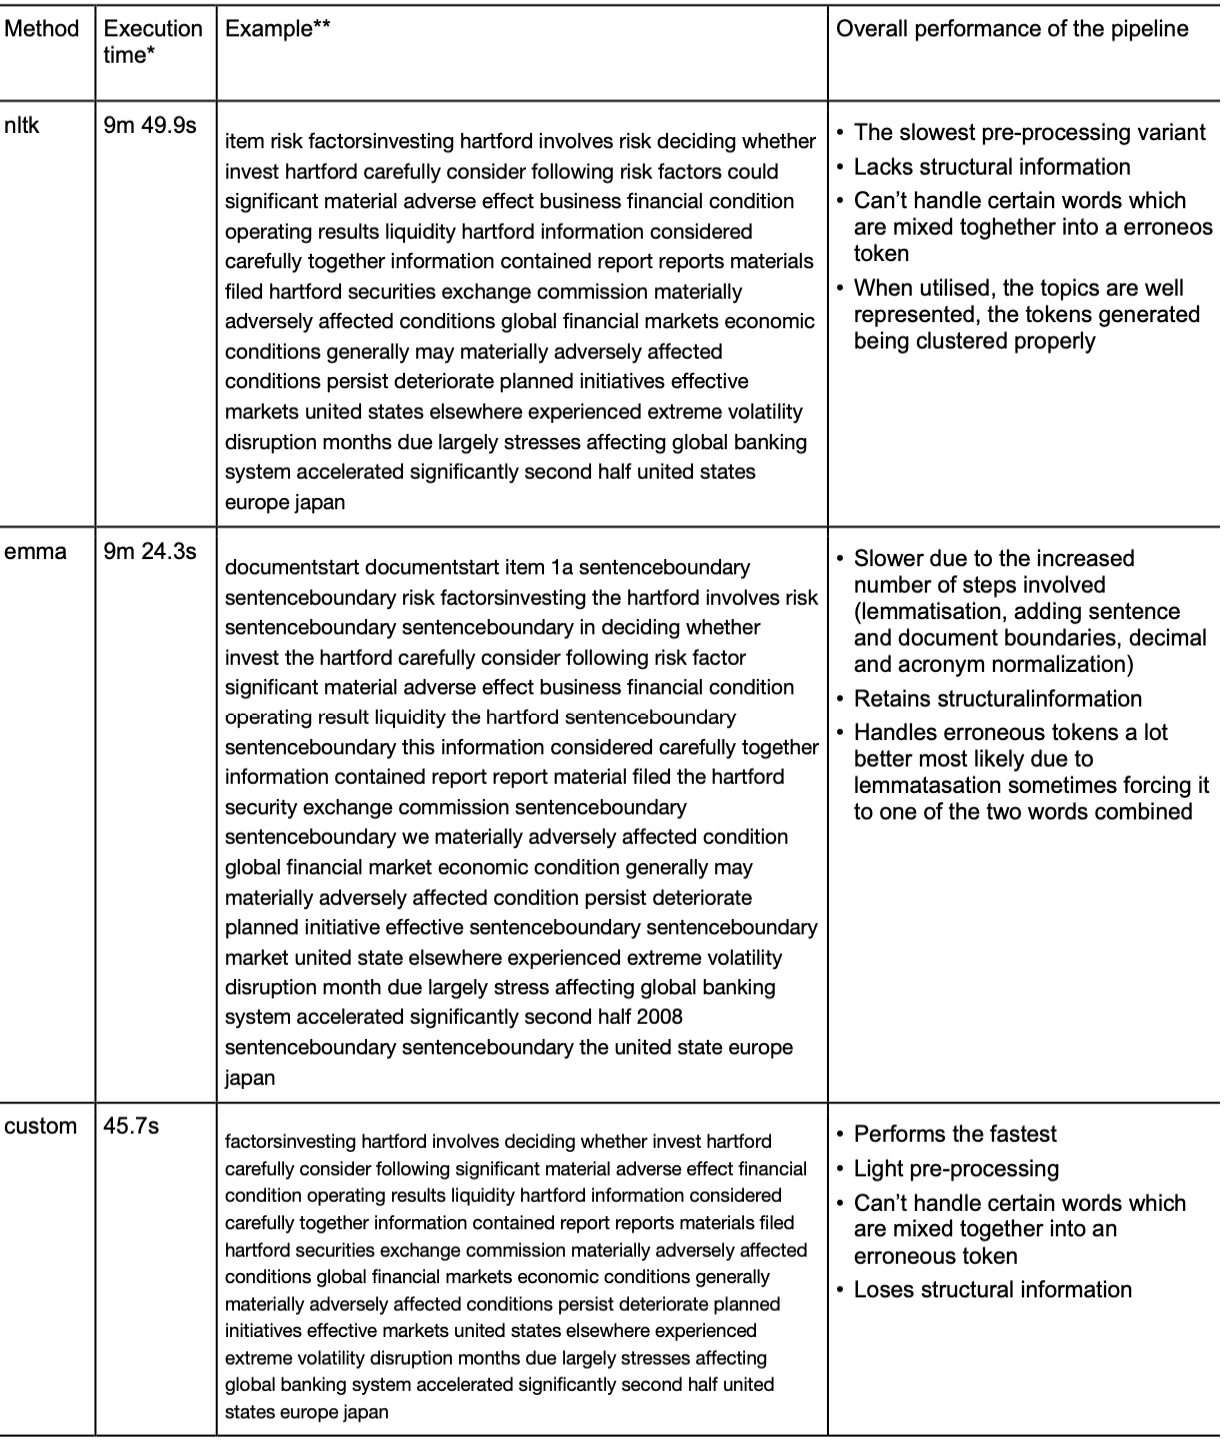
\includegraphics[scale=0.52]{images/pre-processing-variantas.png}
    \caption{Qualitative analysis of the pre-processing variants}
\end{figure}

\subsection{BERTopic}
To use the BERTopic pipeline, I utilised the library created by \cite{grootendorst2020bertopic} with the same name.
The implementation can use MongoDB instances and local data from a CSV file. There are also two more filtering options, one based on start\_year and end\_year, and one based on size, size\_cutoff. The cleaning\_method parameter chooses one of the pre-processing approaches explained above. 
Regarding the actual BERTopic library, in my adaptation of the implementation, there are multiple parameters added to choose from to tune the performance and output:
\begin{itemize}
    \item embedding *i: this parameter is used to decide on the library utilised for the pre-trained sentence embedding by BERT. There are multiple options listed on the official documentation(\cite{bertopic-embeddings}). From those, I decided to implement 4 (Gensim was excluded directly due to mention on the official documentation, regarding its use case intended more for shorter documents, which is not the case here):
    \begin{itemize}
        \item sentence-transformers: Utilises Sentence Transformers from Hugging Face. You can load any pre-trained embedding(\cite{huggingface-models}).
        \item  flair(\cite{flair-nlp}): An advanced library for NLP. It works with the same pre-trained models from Hugging Face. 
        \item spaCy: spaCy is a fast library written for Python and Cython. This comes with their models, based on transformers(\cite{DBLP:journals/corr/VaswaniSPUJGKP17}) architecture.
        \item USE: Universal Sentence encoder provided by Google via their pre-trained model platform, TensorFlowHub. This utilises TensorFlow technologies in the backend.
    \end{itemize}
    \item model\_complexity *i: This parameter is used to decide the granularity of fine-tuning for the BERTopic pipeline line used. There are three levels:
    \begin{itemize}
        \item default: it uses all the default parameters of BERTopic to extract the topics
        \item  custom: it allows for several fine-tuning parameters of BERTopic, without the need to instantiate submodules manually. The options available are:
        \begin{itemize}
            \item n\_gram\_range: the n-gram range that will be used to create a token out of
            \item top\_n\_words: the number of words with the highest score that should represent a topic
            \item nr\_topics: To achieve a specific number of topics (this depends on the pre-trained embedding you select. Specific models can generate more topics than others, which will not artificially increase the search to accommodate a higher number. There is a limited interval of expansion.
            \item low\_memory: option passed further down to UMAP submodule to utilise an algorithm less memory intensive, bypassing hardware limitation
        \end{itemize}\\
        \item Full: it instantiates every submodel utilised in the pipeline. For each one of the submodules, there are specific parameters that you can use to influence the performance and results (this includes the previously mentioned parameters from the custom run. Initially, this had all the possible parameters offered by the following libraries. However, after experimentation, only several of them would produce any meaningful difference without rendering the results useless):
        \begin{itemize}
            \item UMAP specific hyperparameters:
                \begin{itemize}
                    \item n\_neighbours:As n\_neighbors is increased, UMAP manages to see more of the overall structure of the data, glueing more components together and better coveying the broader system of the data(\cite{umap-parameters}). In practice, for this use case, the range in which this performs best is 10 to 20, determined during the experimentation phase. Keeping topics isolated will lead to uncorrelated results. Increasing it past 20 would lead to more similar clusters, losing differences and potential subtopics of a more important topic.
                    \item n\_components: parameter to decide the dimensionality of the space to which each embedding is reduced. For visualisation purposes, this can be used as low as 3. However, for HDBSCAN to perform better, it needs to strike a balance between more dimensions(making more data available and retaining local information) and performance(when used with n\_components to 50, the pipeline would crash due to filling up the RAM on all configuration tested). When manually experimenting with this parameter, I observed that the best value is around 10. However, it should perform similarly if greater than 5 and less than 20.
                    \item Cannot handle certain words which are mixed toghether into a erroneos token
                    \item Loses structural information
                \end{itemize}
            \item HDBSCAN specific parameters:
                \begin{itemize}
                    \item min\_cluster\_size: Minimum number of points needed to create a cluster. This is a specific parameter, but it can have strange behaviours if not used correctly(more details[48]). The value that performed best for me is to set it somewhere between 10 and 20, with less than that range creating too many clusters, which are not representing anything in particular. More than 20 would lead to too few clusters being formed, most of the points being considered as noise.
                    \item min\_samples: the parameter that decides how conservative the clustering is.(\cite{McInnes2017}) In the experiments that I ran, the best value by far was 1. Any number greater than 3 would drastically reduce the number of topics generated, many of them being considered noise directly. Using certain embeddings (USE from tensorflowhub) allows the use of the number of samples as 2 because it can generate a lot more topics than the rest options.
                    \item metric: the metric used to determine the distance between data points in high dimensional space while clustering. All the data distance metrics from sklearn(\cite{scikit-learn}) are available. In this case, after researching the problem(\cite{Aggarwal2001OnTS}), I decided to utilise the Manhattan distance
                    \item prediction\_data: This will save all the probabilities used to determine the most likely cluster. Even though this data is not explicitly used in later stages of the pipeline, without it, BERTopic does not output the proper format for the topics later used in the DTM method.
                \end{itemize}
            \item nr\_topics: To achieve a specific number of topics (this depends on the pre-trained embedding you select. Specific models can generate more topics than others, which will not artificially increase the search to accommodate a higher number. There is a limited interval of expansion.
            \item low\_memory: option passed further down to UMAP submodule to utilise an algorithm less memory intensive, bypassing hardware limitation
        \end{itemize}
    \end{itemize}
\end{itemize}
*i = These parameters were implemented specifically for this pipeline, they are not part of the underlying libraries used. \\
After obtaining the topics from the topic model generated with BERTopic, we can visualise several stats about them, such as topic clusters, topic hierarchy, and topic similarity, and analyse the performance.
The initial approach was to run all the models using only the default method with the same pre-trained model. However, several key differences between different libraries, hyperparameters, and models were used. I ran four experiments, for each model, with the same dataset, exact configuration, different pre-trained embeddings and different hyperparameters.

\begin{table}[h]
  \caption{Experiments performed to determine different's library performance}
  \label{tab:experiments}
  \begin{tabularx}{\textwidth}{|X|X|X|X|X|}
    \toprule
    {Parameters}&{Experiment 1}&{Experiment 2}&{Experiment 3}&{Experiment 4}\\
    \midrule
    Model complexity & Default & Default & Custom & Full\\\hline
    Embedding & Fastest available* & Best performing available** & Fastest available* & Best performing available**\\\hline
    No topics required & None specified & None specified & 800*** & 800*** \\\hline
    Pre-processing variant & custom & custom & custom & custom\\
  \bottomrule
\end{tabularx}
\end{table}

\begin{table}[h]
  \caption{Pre-trained models used by each library for each experiment}
  \label{tab:pretrained-models}
  \begin{tabularx}{\textwidth}{| X  X  X  X  X |}
    \toprule
    {Library}&{Experiment 1}&{Experiment 2}&{Experiment 3}&{Experiment 4}\\
    \midrule
    sentence-transformers & all-MiniLM-L6-v2 & all-mpnet-base-v1 & all-MiniLM-L6-v2 & all-mpnet-base-v1\\\hline
    flair & all-MiniLM-L6-v2 & all-mpnet-base-v1 & all-MiniLM-L6-v2 & all-mpnet-base-v1\\\hline
    tensorflow_hub & universal-sentence-encoder-lite  & universal-sentence-encoder  & universal-sentence-encoder-lite  & universal-sentence-encoder \\\hline
    spaCy & en\_core\_web\_sm & en\_core\_web\_trf & en\_core\_web\_sm & en\_core\_web\_trf\\
  \bottomrule
\end{tabularx}
\end{table}

For best performance, while not the actual aim of this topic modelling task,"Performance Sentence Embedding"(\cite{DBLP:journals/corr/abs-2101-10642}) was used as a metric to measure it. \\
* When selecting the fastest available, I mean picking the model with the best performance which runs the fastest according to testing completed by third parties (\cite{grootendorst2020bertopic}, \cite{sbert-models}). \\
** When selecting the best performing available, I mean the one who scored the highest in Performance Sentence Embeddings and I was able to run (some of the best performing models require better hardware which I did not have access to) \\
*** The number 800 was selected by running the pipeline multiple times and looking at the highest value achievable on average without losing the relevance of topics. This rationale will become important later when utilising these topics for Dynamic Topic Modelling. A topic's relevance in this context refers to how much information is enclosed in that topic. \\
For example, there are topics which do not offer any value they are formed just based on their embeddings having a high similarity degree \\ (topic 147\_companys\_company\_financial guaranty, which was created by the following tokens:" companys, company, companys financial, companys products, company busines"), and there are topics which reveal unexpected connections(topic 699\_loans\_bank\_sba\_open bank which was defined in 2007 by the following tokens: "cbi, cbi merger, merger, southern california, ban" refers to the Chicago Bridge & Iron buying Lummus Global business, a provider of process technologies (\cite{topic-modelling-example}).They disclosed the risk involved in this takeover, alongside the loans to solidify the needed cash flow. When tracking the evolution of the topic, the struggles that followed due to the financial crisis and the rising interest rates are easily trackable. This ground kept this topic increasing in the risk section to its local maximum in 2011 and decreasing afterwards).
The dataset was made up of 2789 documents instead of the complete one to attenuate the duration of the benchmarking experiment. The topic number will not reach 800 due to the limited number of topics. However, the better performance would be considered the one with the most topics. The tests were performed on configuration C.
The following is a comparison between the different combinations tested and the results coupled with several observations:
\begin{figure}[h]
    \centering
    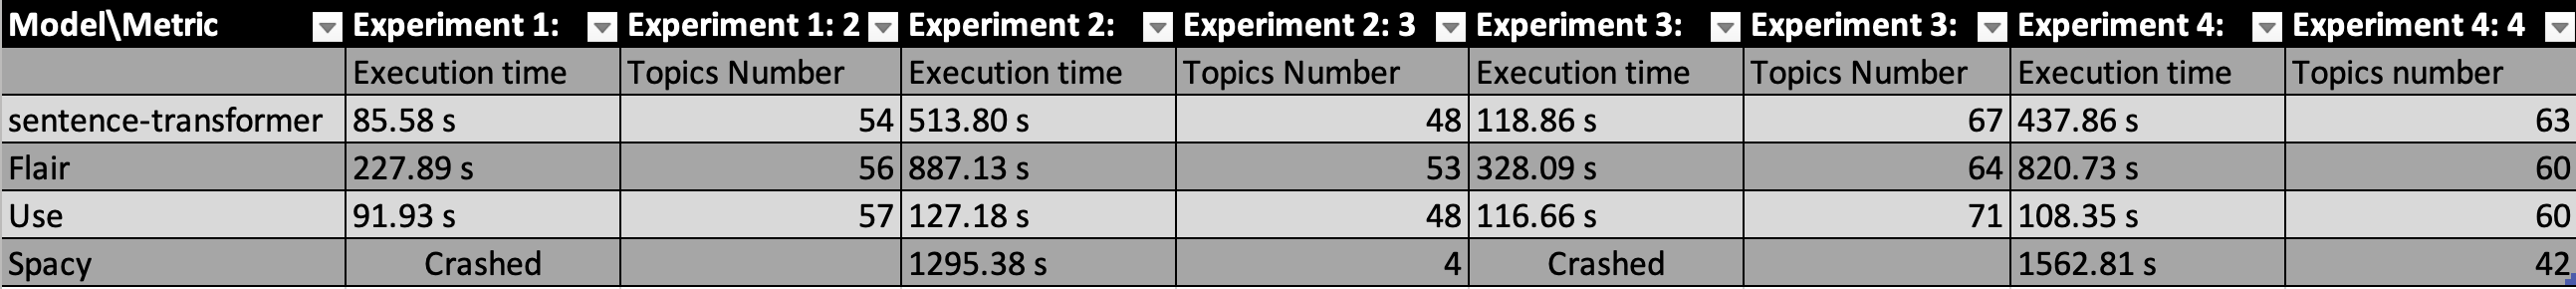
\includegraphics[scale=0.37]{embeddings_comparasion.png}
    \caption{Experiments performed to compare the different libraries with different pre-trained models}
\end{figure}

Several conclusions can be drawn from the experimentation phase:

\begin{itemize}
    \item Optimised hardware and environments must be used with a benchmarking framework to test and evaluate these differences properly. I was limited by a consumer-grade configuration's computing power and reliability issue in performing these experiments.
    \item Most of the best performing models are available on the HuggingFace platform(\cite{huggingface-models}). However, not all libraries used for embedding support them. For spaCy and USE(Tensorflow), I tried my best to match the characteristics of the pre-trained models to maintain the comparison relevance.
    \item  sentence-transformer and flair are interoperable, offering access to all the models available on the HuggingFace platform. Flair also has several bespoke models built for it. However, they performed roughly the same in my testing, with noticeable decreased performance. At the same time, the sentence-transformer was faster on average, especially on more powerful configurations such as A, B and E. Flair allowed to run any model on any configuration without any reliability issues. If compatibility and reliability are the goals, I recommend using the latter.
    \item The best performing and optimised encoding library was USE (based on Tensorflow). However, this also resulted in the most crashes and reliability issues. The representations offered by this variant performed significantly better later on in the pipeline, mainly when used in the time-series forecasting model.
    \item Even though this is not an exhaustive analysis, spaCy was the worst performer in this experimentation phase. It outputted the most irrelevant topics, failing most of the time to comply with the number of topics requested and performing the poorest no matter the configuration or the optimisations undertaken.
\end{itemize}\\


After obtaining the topics and probabilities matrix, the results, due to a lack of a benchmarking framework, were evaluated on Term Score Decline, Topic Similarity and random sampling to determine relevance.
One strange behaviour noticed in this implementation of BERTopic was that negative topics would be used to cluster erroneous, or in some cases too broad, terms and topics. These entries would be removed from the final results.
The following pipeline step is to model these topics over a timeframe. This is done via the built-in functionality of BERTopic to utilise DTM. There are two parameters to be considered when running the "topics\_over\_time" method:

\begin{itemize}
    \item global\_tuning: This option allows each topic's representation to be adjusted by the overall global representation. In principle, this sounds like a valid extension. However, we consider topics independent (at most being influenced by nearby or hierarchically lower clusters). This is an example of how this affects the end product (\ref{appendix:9}1, \ref{appendix:10}2). The final output is not severally impacted, on average, by 1.74 points on the frequency scale. However, I decided to set this parameter to False.
    \item  evolution\_tuning: This option allows tuning each topic's representation at a specific timestamp with the previous one. Throughout the entire pipeline, this option was set to True, the desired effect.
\end{itemize}

The entire implementation of the aforementioned BERTopic approach can be found in the bertopic\_model.ipynb file. The end product of this part of the pipeline will be a tabular file, in a .csv format, which contains multiple time series, one for each topic, tracking their evolution over the timeframe. (\ref{appendix:11}3, \ref{appendix:12}4). This will represent the dataset for all the other machine learning models implemented. It is imperative to balance the number of topics against relevance. The more relevant topics there are, the better it is.

\subsection{Classifier model to determine if a topic is going to raise or not}


The first idea that I attempted with the newly generated dataset was to build a classifier which would determine if a topic would increase or not in importance(frequency). This can be labelled as a binary classification task. The first step was creating two new columns for the dataset "Frequency\_Next\_Year" by shifting the Frequency column to "is\_growing", defined by the difference between frequencies next year and current. After analysing multiple results, I observed a ratio of 3:1 between data points, represented by topics at a specific timestamp, which make up the two classes. For example, for a DTM dataset generated by flair with an n-gram range of 2, there are 772 topics over 15 timestamps. The "increase in importance" subset is represented by 2392 data points, while the other class has 6637. 
The next step was Feature engineering. The dataset generated by DTM only includes the topic, topic's tokens, frequency and timestamp. Even though there are multiple guides (\cite{basic-fea-timeseries}, \cite{fea-timeseries}, \cite{a-guide-to-feature-engineering-time-series-tsfresh}) and research in the area of engineering features from time series(\cite{Tang2020EnrichingFE}), there is nothing in-depth to analyse the performance impact of including tokens or tokens embeddings in it. There are two types of features that this model uses:
\begin{itemize}
    \item General time-series features:
        \begin{itemize}
            \item Lag-1: the value of the frequency of the topic one timestamp before
            \item Topic number: helps in tracking the evolution of a topic through time
            \item Diff-1: the difference between the frequency at timestamp t and timestamp t-1
        \end{itemize}
    \item Features used in \cite{Tattershall2019DetectingBT}:
        \begin{itemize}
            \item Rolling-4,8: moving average of the frequency values on the previous 4 and 8 years
            \item MACD: obtained using Rolling-8 and Rolling-4 difference
            \item Signal: moving average of the MACD values over the last 2 timestamps
            \item Hist: (Histogram) difference between MACD and the Signal columns
        \end{itemize}
\end{itemize}

\begin{figure}[h]
    \centering
    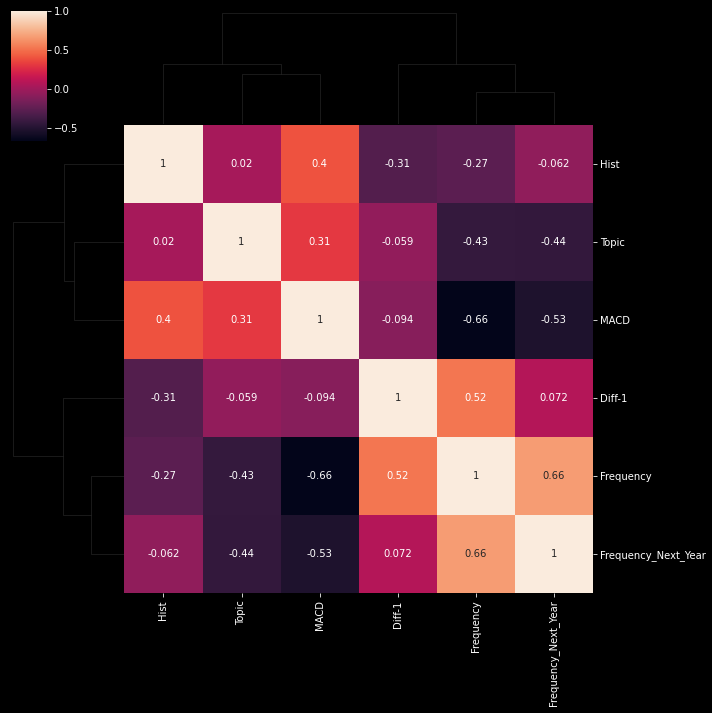
\includegraphics[scale=0.5]{test_corelatie.png}
    \caption{Correlation heatmap between the features selected and the target variable 'Frequency\_Next\_Year}
\end{figure}

\newpage

Legend for the feature visualisation figures : 
\begin{itemize}
    \item The shape of the point = is\_growing (circle=True, square=False)
    \item Colour of a point = Topic number (Starting from the first topics visible in a darker blue to bright yellow the last topics)
    \item Size of the point = Frequency (The higher the frequency, the bigger the data point)
\end{itemize}

\begin{figure}[h]
    \centering
    \subfigure[1]{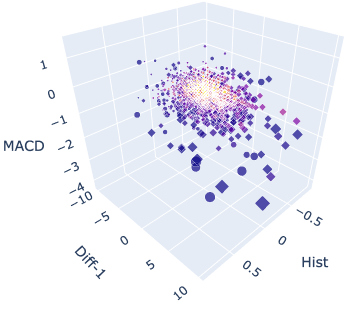
\includegraphics[width=0.45\textwidth]{dataset_analysis/3d_features_slot.png}} 
    \subfigure[2]{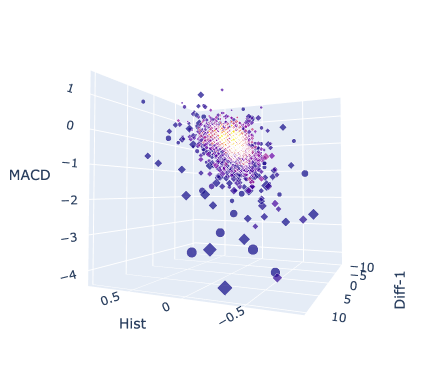
\includegraphics[width=0.45\textwidth]{dataset_analysis/Classifier_plot.png}} 
    \subfigure[3]{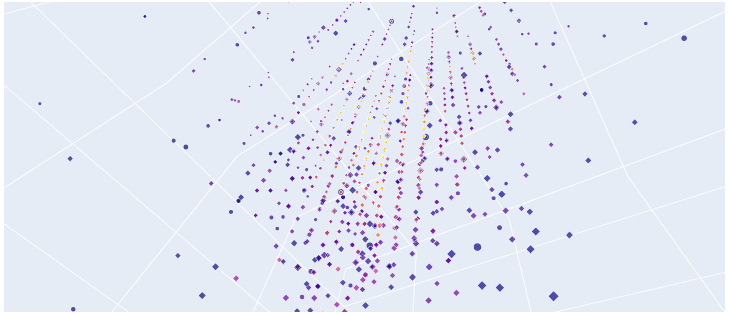
\includegraphics[width=0.45\textwidth]{dataset_analysis/deep_dive.png}}
    \caption{Visualisation of the features in the form of a 3D Scatter Plot}
    \label{fig:foobar}
\end{figure}

\newpage

Based on the previous views, we can observe several patterns:
\begin{itemize}
    \item Earlier topics are more spread outwards and generally more significant in size.
    \item The data points are indistinguishable from the point of view of the two classes that they need to be fitted in 
\end{itemize}
 
I initially implemented a RandomForrestClassifier provided by sklearn(\cite{scikit-learn}). This was barely reaching 0.5 precision in both classes, so I had to change it for better-suited models for unbalanced data. To tackle this issue, I tried both undersamplings, which negatively impacted the results, and oversampling, using SMOTE (\cite{JMLR:v18:16-365}), which slightly improved the overall accuracy.
The final models implemented are SVC, GradientBoostingClassifier and AdaBoostClassifier.
There is also a separate way in which the topic number column was encoded using an OneHotEncoder to remove the potential hierarchical bias that the model can develop.
I used a 90/10 split of the dataset for each model and a 10-fold cross-validation to ensure reliable results.

\subsection{Prediction models}
\subsubsection{Timeseries forecasting model}

Considering the output generated by DTM, I decided to utilise a popular time-series forecasting library, DARTS(\cite{herzen2021darts}). This library has multiple ways to import data. After conversion, it is ready to use many models for prediction tasks. In this case, the model needed to support multiple-series training. Each topic will be treated independently, resulting in multiple time series being fed during the training phase. From the long list of models available, I experimented with RandomForest, RNNModel, TCNModel and NBEATS model.
The implementation is available in timeseries\_model.ipynb. It loads a local tabular file containing the output of DTM. I implemented a convertor which takes the topics column and splits it into the desired objects required by the library. Afterwards, the data would be divided into a 90/10, where 90\% of the time series were used for training and 10\% for testing.
 
Even though I tried multiple configurations and combinations of hyperparameters, the shortcoming of this approach became clear very fast; the time series was too short. Even on a relatively simple test such as historical forecasting on specific sample topics, the R2 score would be considerably low, whereas the MAPE would constantly be high:

\begin{figure}[h]
    \centering
    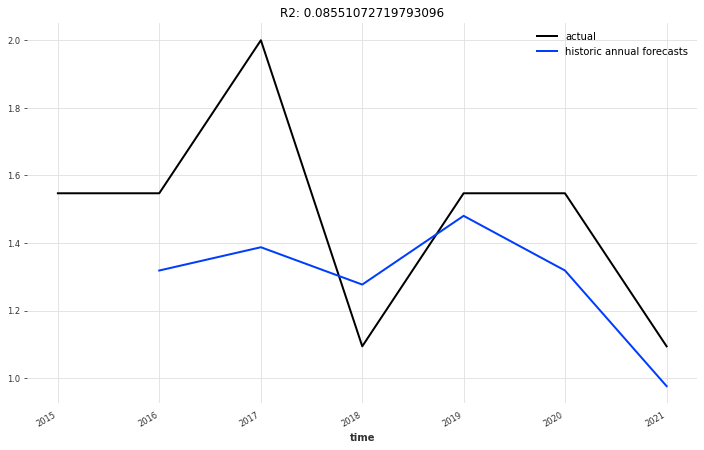
\includegraphics[scale=0.3]{timeseries_forecasting_best_case_scenario.png}
    \caption{The best-case scenario for time-series forecasting: MAPE 15,51\%}
\end{figure}

\begin{figure}[h]
    \centering
    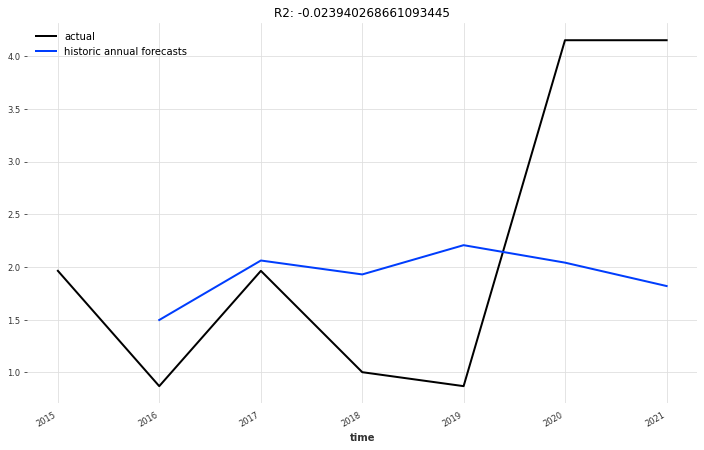
\includegraphics[scale=0.3]{timeseries_went_wrong.png}
    \caption{Timeseries forecasting poor performance: MAPE 71.70\%}
\end{figure}

	 
There are two approaches to fix this problem: changing the frequency of the time series by analysing quarterly reports or expanding the dataset with more years to be processed from the beginning.

\subsubsection{Regression model}
The last model that I developed was a regression model to predict the importance of a topic. I decided to utilise a RandomForestRegressor from the sklearn library (\cite{scikit-learn}). This underwent the same feature engineering steps as the classifier mentioned above.  However, different features were selected in the end for this approach. MACD, Signal, Rolling-8 and Hist were removed from the previously mentioned features. Even though the correlation matrix with the target value pointed out that there is value in keeping them, the results in practice showed that they hindered performance.
Moreover, compared to the initial approach, I tried embedding the top 5 tokens representing a topic and passing them as features again. However, the correlation looked weak for this attempt, with only the first words achieving a -0.075 in the best-case scenario with the target variable. A logging system was implemented for each train and testing run I performed. Also, when splitting the data, I decided to implement multiple approaches due to the unclarity in the literature about how K fold validation should work for regression over time series. The previously used ratio of 90/10 was kept for this implementation too. When plotting a distribution of entries based on the importance of one timestamp, you could see that roughly 90\% of data points were placed at intervals between 0-4, with another 5\% in the 5-9 range. This meant that both my attempts at normalising the data were futile, and a better idea would be to remove the very few outliers, which I did in one of the experiments.
Before I did any experimenting, I performed a thorough hyperparameter tunning for every parameter sensible to this model, choosing the best one based on the lowest RMSE score, the highest R2 score (which would have been my first choice if there weren’t any reliability issues when the values are very low) and the shortest execution time. 
In the first experiment, I used OneHotEncoder over the “Timestamp” and “Topics” columns, intending to obfuscate the hierarchical dimension of this data. The split is made randomly in 10 folds, without maintaining the ratio for each topic in particular.
In the second experiment, I only used the engineered features, and the data were evenly split per topic, keeping the same ratio.
In the last experiment, I kept the features from the previous experiment but randomly shuffled the entire dataset before splitting it into train and test.
Each experiment was run with and without outliers, a parameter available for changing.

\subsection{Evaluation Metrics}

When it comes to evaluating the performance of the pipeline, there is no clear, objective metric to track the progress. The definition of importance is its quality of being significant, valued, or necessary in a particular situation. The description of a \textit{topic} is the subject of discourse. The importance of a topic is a subjective measure. For example, suppose we use the analysis to evaluate the stock market's performance. In that case, importance can be seen as relevant to predicting risks and companies that would be impacted: "Something (A) is relevant to a task (T) if it increases the likelihood of accomplishing the goal (G), which is implied by T."(\cite{Hjrland2002WorkTA}). When utilising DTM, the best representation of this abstract concept is derived from frequency for this specific case. A topic is more important and relevant for the market or the business environment, as it increases throughout multiple documents from multiple firms over various timestamps.
I also performed a qualitative analysis of the results, from which I drew several observations.
 
Moreover, for each specific machine learning model developed, I used task-specific metrics:
\begin{itemize}
    \item Classifier model:
    \begin{itemize}
        \item Precision: \cite{wiki:p&r}
        \item Recall: \cite{wiki:p&r}
        \item F1-score: \cite{wiki:f-score}
    \end{itemize}
    \item Regression model:
    \begin{itemize}
        \item Root mean squared error (MSE): \cite{wiki:mse}
        \item Mean absolute error (MAE): \cite{wiki:mae}
        \item Mean absolute percentage error (MAPE): \cite{wiki:mape}
        \item Coefficient of determination (R2): \cite{wiki:r2}
    \end{itemize}
    \item Timeseries forecasting model:
    \begin{itemize}
        \item Mean absolute percentage error (MAPE): \cite{wiki:mape}
        \item Coefficient of determination (R2): \cite{wiki:r2}
    \end{itemize}
\end{itemize}
All the observations mentioned above and metrics will be accompanied by plots and figures to visualise the results better. 

\chapter{Results}

\section{BERTopic Results}
One significant limitation of BERTopic is that it requires an extensive dataset to output meaningful results. With limited and sampled sub-datasets, the topics would converge around the same general ideas (banks, loans, reporting, crisis, technology, legal, fee, commission, legislation).
The library offers a plethora of visualisation options for this model. However, the Term Score Decline is the best one for determining the relevance of the topics generated using different pre-trained models and settings. Topics are a cluster of tokens(representing words or n-grams) associated with a c-TF-IDF. To form this kind of group, you start with the best matching word, or the founding word depending on the topic modelling algorithm that you choose, and start adding words that are the closest to the topic or domain while at the same time broadening the spread and meaning of it. After an upper limit, any word added would not significantly impact the c-TF-IDF. It would only pollute the representation built so far. This visualisation is powerful because it allows us to interpret how those topics were formed easily. During my qualitative analysis, a clear trend, which cannot be captured in any objective measure, was that topics with a slower term score decline, with words more closely related together, were more relevant.
These are the term score decline charts for the all the possible libraries, using the default configurations, with the best performing pre-trained models.

\begin{figure}[h]
    \centering
    \subfigure[a]{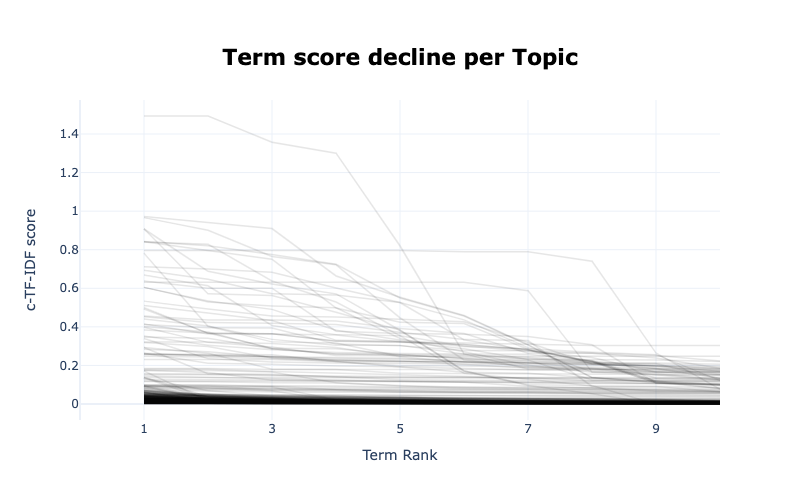
\includegraphics[width=0.4\textwidth]{results/sentence_transformers_term_score_decline.png}} 
    \subfigure[b]{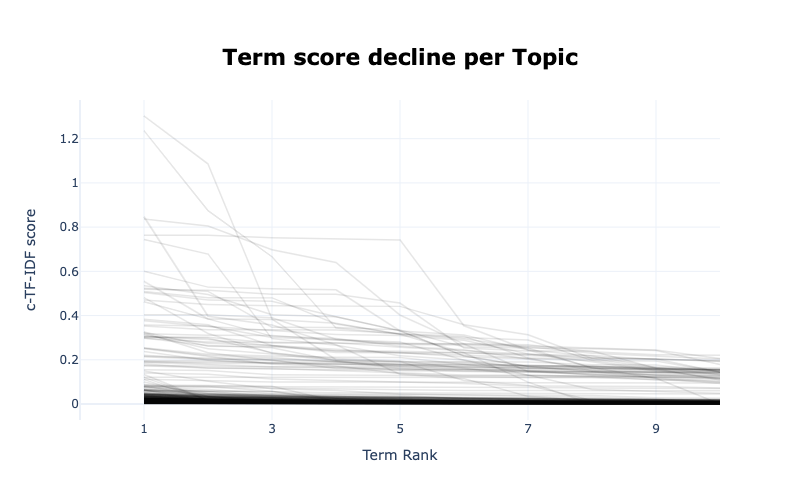
\includegraphics[width=0.4\textwidth]{results/flair_term_rank_decline.png}} 
    \subfigure[c]{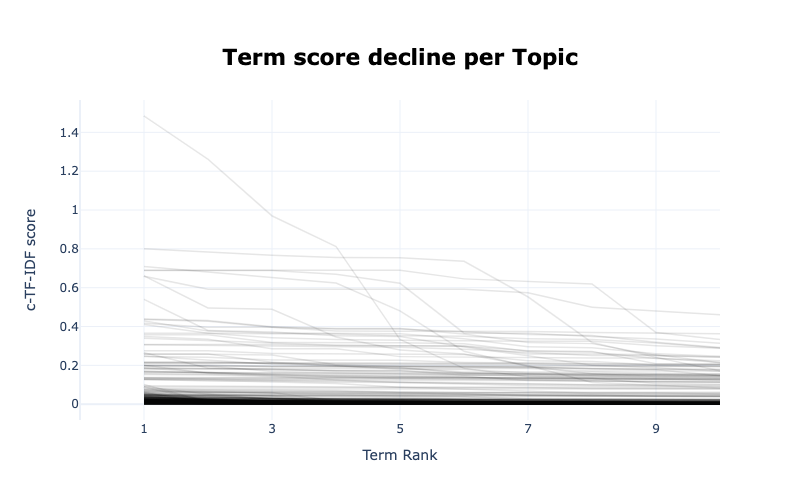
\includegraphics[width=0.4\textwidth]{results/Term_Score_Decline_USE.png}}
    \subfigure[d]{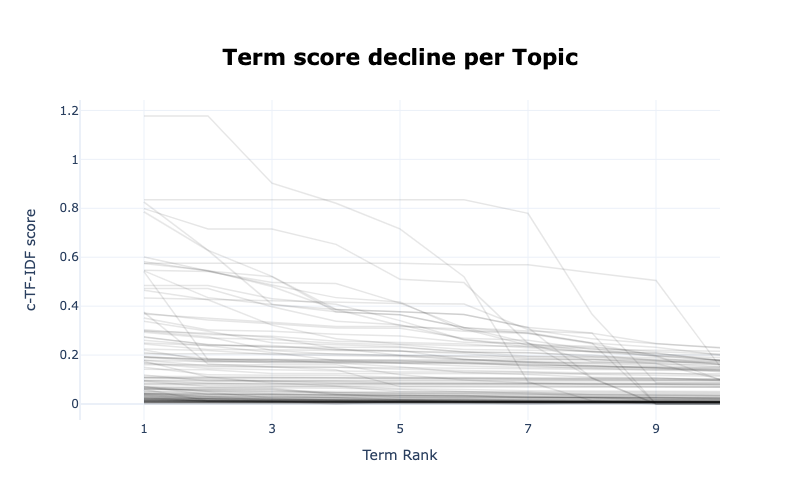
\includegraphics[width=0.4\textwidth]{results/spacy_term_decline.png}}
    \caption{Term score decline performance of (a) sentence-transformers (b) flair (c) tensorflow\_hub (d) spaCy}
    \label{fig:foobar}
\end{figure}

Based on this analysis, we can observe a clear better performer in spaCy. The only problem would be the number of topics outputted by it, around 100 less than the others, contributing to the advantage. The worst performer by far was USE, the topics generated being relatively coherent. However, it lacks the resulting probabilities to back up that impression with data.
The second visualisation test that I employed to decide which library to use was the intertopic distance map. This shows where the topics are located in a two-dimensional space. While this is not a faithful exemplary representation, the desired behaviour is for the clusters to separate without overlapping. These are the cluster views for all the models tested, in the same configurations as before.

\begin{figure}[h]
    \centering
    \subfigure[a]{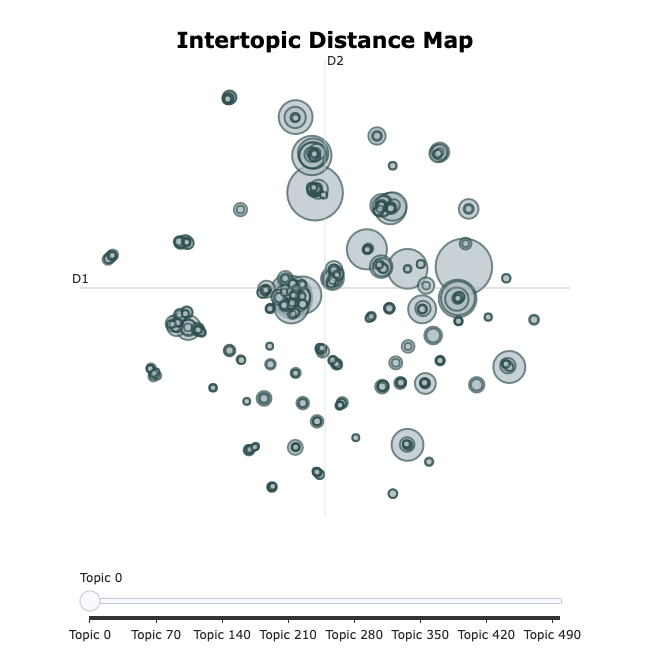
\includegraphics[width=0.4\textwidth]{results/Cluster Sentence Transformers.png}} 
    \subfigure[b]{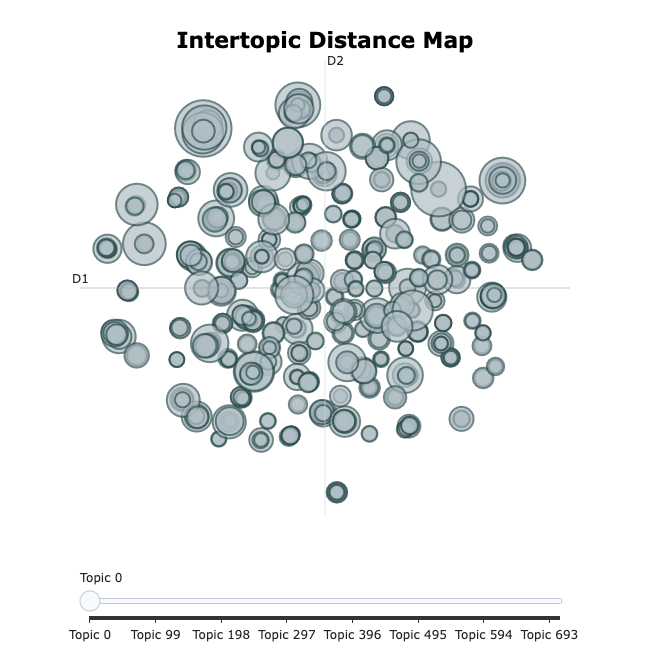
\includegraphics[width=0.4\textwidth]{results/flair_longest_run.png}} 
    \subfigure[c]{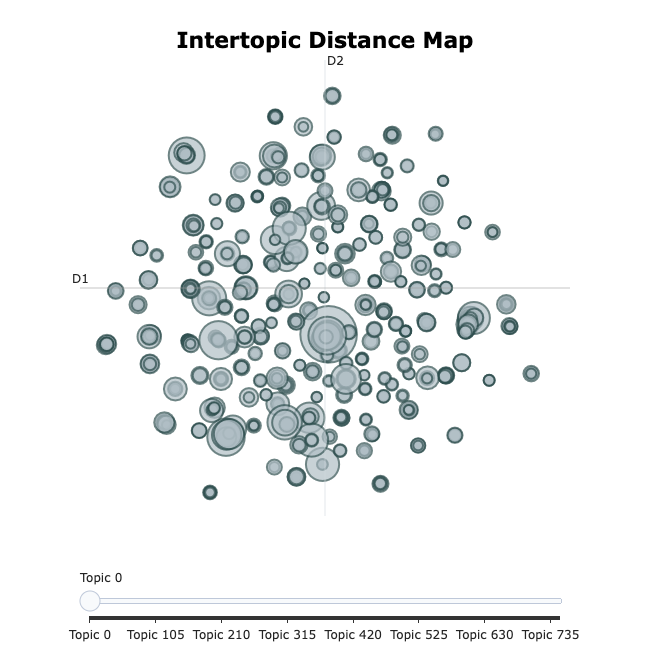
\includegraphics[width=0.4\textwidth]{results/CLusters_topics_use.png}}
    \subfigure[d]{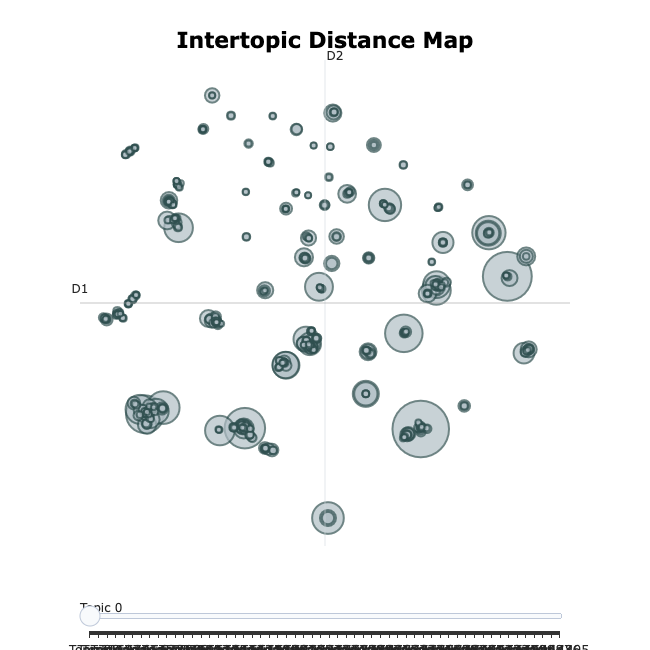
\includegraphics[width=0.4\textwidth]{results/Clusters of Topics spaCy.png}}
    \caption{Term score decline performance of (a)sentence-transformers (b)flair (c)tensorflow\_hub (d)spaCy}
    \label{fig:foobar}
\end{figure}

There are two standout performers from this second visualisation: flair and tensorflow\_hub. The shortcoming of spaCy strikes again, its clusters being sparse and overlapped. On the other hand, sentence-transformers suffer from a different problem, over-specialisation. The clusters are minimal, meaning that the samples supporting those topics are at a bare minimum for them to be categorised as a cluster in the first place.

However, the main target of using BERTopic is to take those topics and use them with DTM to obtain time series for each topic to track their evolution. Based on the previous two tests, I decided to use the sentence-transformers library with the pre-trained model \textit{all-mpnet-base-2} for all the following testing performed with machine learning models. 

\begin{figure}[h]
    \centering
    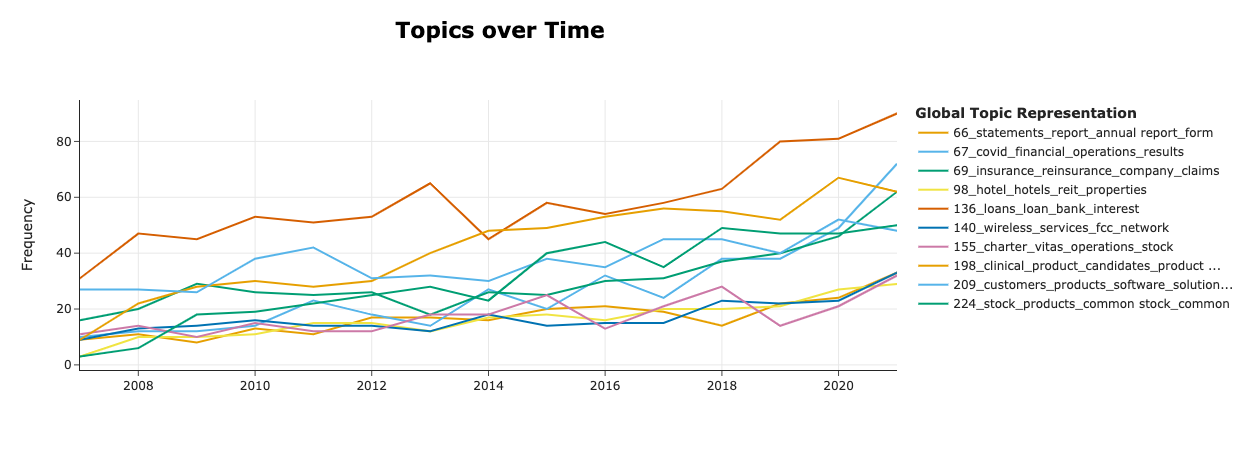
\includegraphics[scale=0.4]{results/tot_longesst_sentence.png}
    \caption{sentence-transformers DTM visualisation: The top 10 topics and their evolution throughout the timeframe used}
\end{figure}

This DTM output of the Risk Factors section is an example of tracking the semiconductors topic occurrences. The spike in 2018 points to the increasing capacity and semiconductor supply chain crisis which hit once the pandemic stopped chip foundries.

\begin{figure}[h]
    \centering
    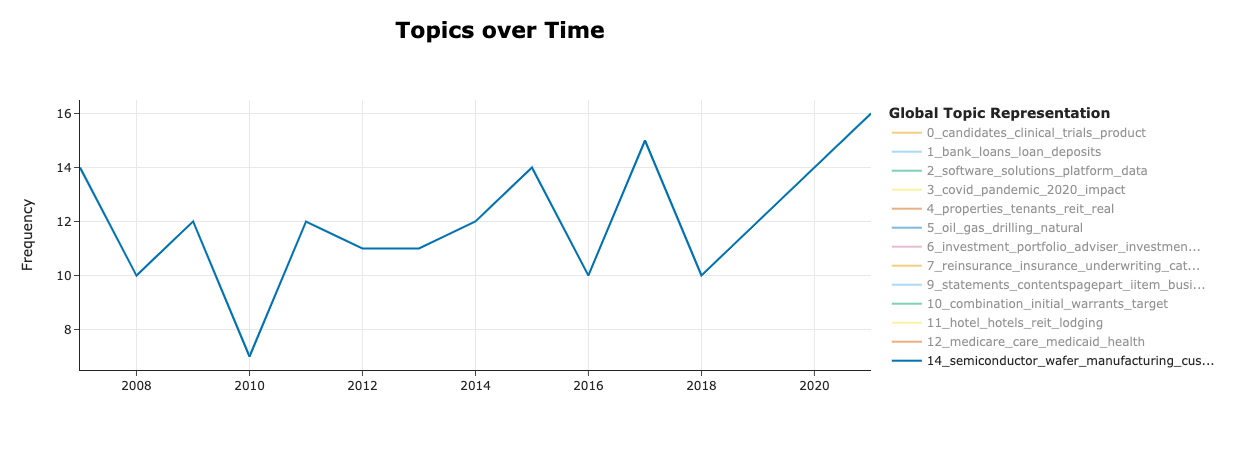
\includegraphics[scale=0.3]{results/topic_evolution_example.png}
    \caption{Evolution of the \textit{semiconductors} topic}
\end{figure}

I also ran one dataset generated from each library for comparison. Still, they are not equivalent because, for USE and spaCy, I had to change the comparable pre-trained model or restrict the dataset, which would not compare to the other two libraries. This measure was enforced by the computing power of all the configurations used: no matter the combination of parameters or optimisations were done, those two libraries would crash before ever finishing.

\begin{figure}[t]
    \centering
    \subfigure[a]{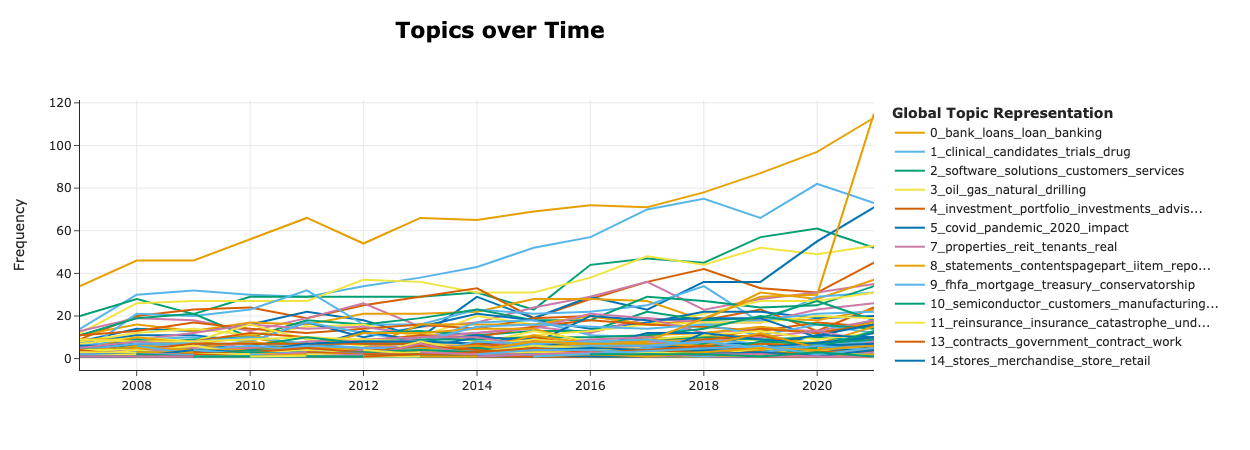
\includegraphics[width=0.5\textwidth]{TOT_without_global.png}} 
    \subfigure[b]{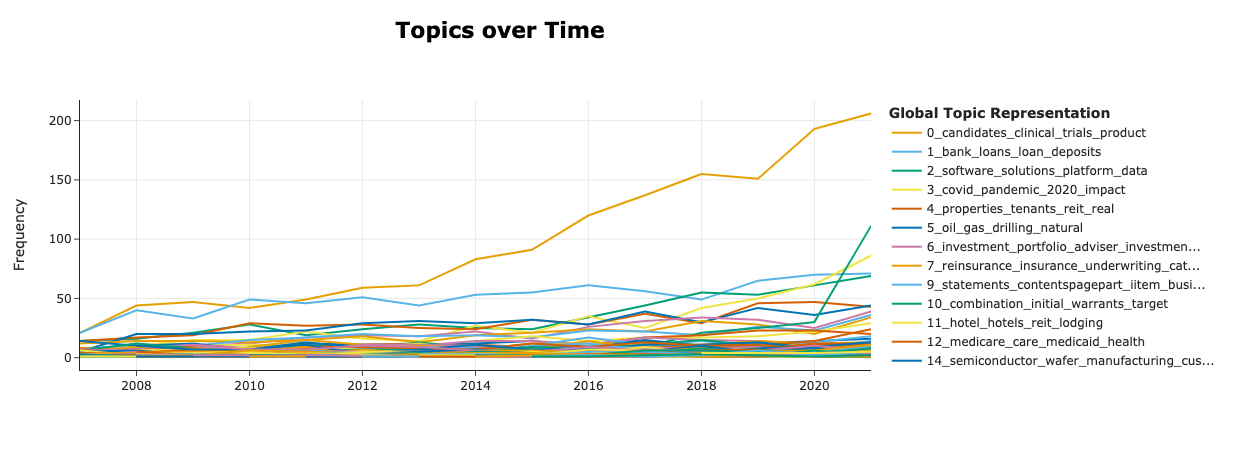
\includegraphics[width=0.5\textwidth]{results/tot-flair-1-3.png}} 
    \subfigure[c]{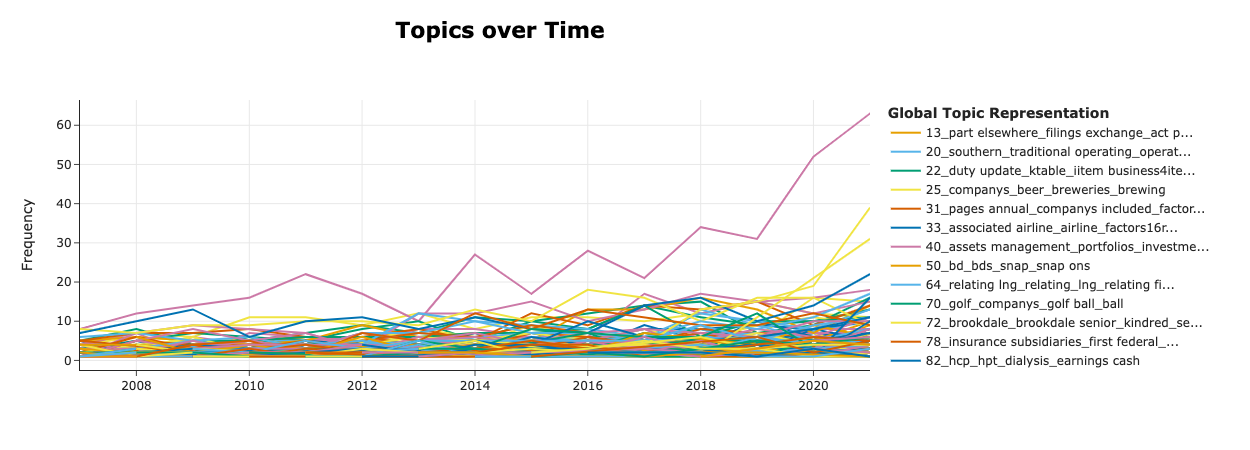
\includegraphics[width=0.5\textwidth]{results/use_tot_latest.png}}
    \subfigure[d]{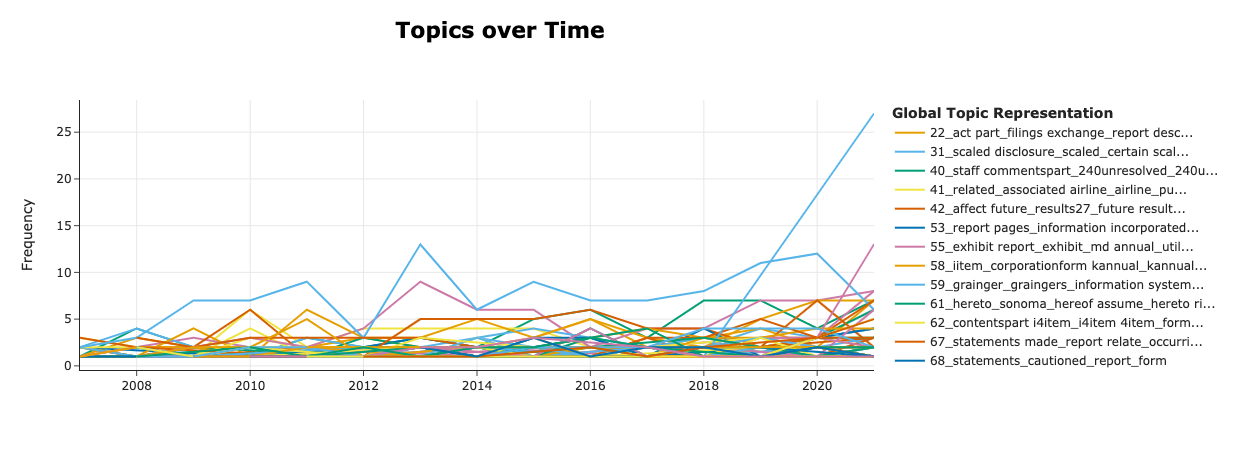
\includegraphics[width=0.5\textwidth]{tot_spacy.png}}
    \caption{Topics over time generated by (a)sentence-transformers (b)flair (c)tensorflow\_hub (d)spaCy}
    \label{fig:foobar}
\end{figure}

The plots are implemented via Plotly, so when analysing the data, you can even interact, single out and dive deeper into the results (\cite{bertopic-online}). This is another example of how topics can be visualized for further qualitative inspection \ref{barchart}.

\begin{figure}[h]
    \centering
    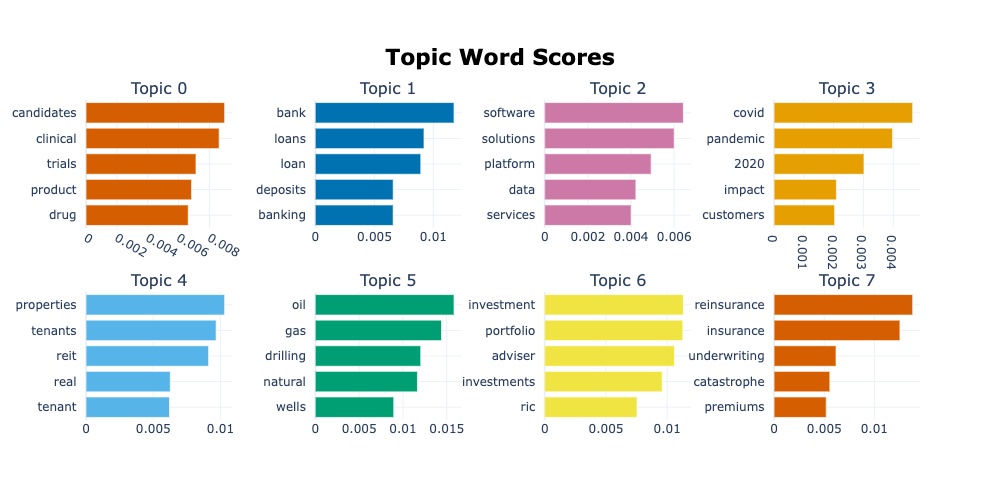
\includegraphics[scale=0.5]{topic barchart flair 1-3.png}
    \caption{Topic bar chart showing the most representative words and their scores}
    \label{barchart}
\end{figure}

These outputs would serve as datasets for the following models developed.
\clearpage

\section{Classifier Results}
The classifier performance can be described as average. It failed in classifying the topics that will grow in importance, having on average a precision insignificantly higher than 50\%. However, for the other category, the precision was overall respectable. The testing was performed using a DTM output obtained with the pre-trained model \textit{all-mpnet-base-2}, used with sentence-transformers, with a full configuration and custom pre-processing. The following table outlines the results based on the multiple combinations of parameters, models and methods.

\begin{figure}[h]
    \centering
    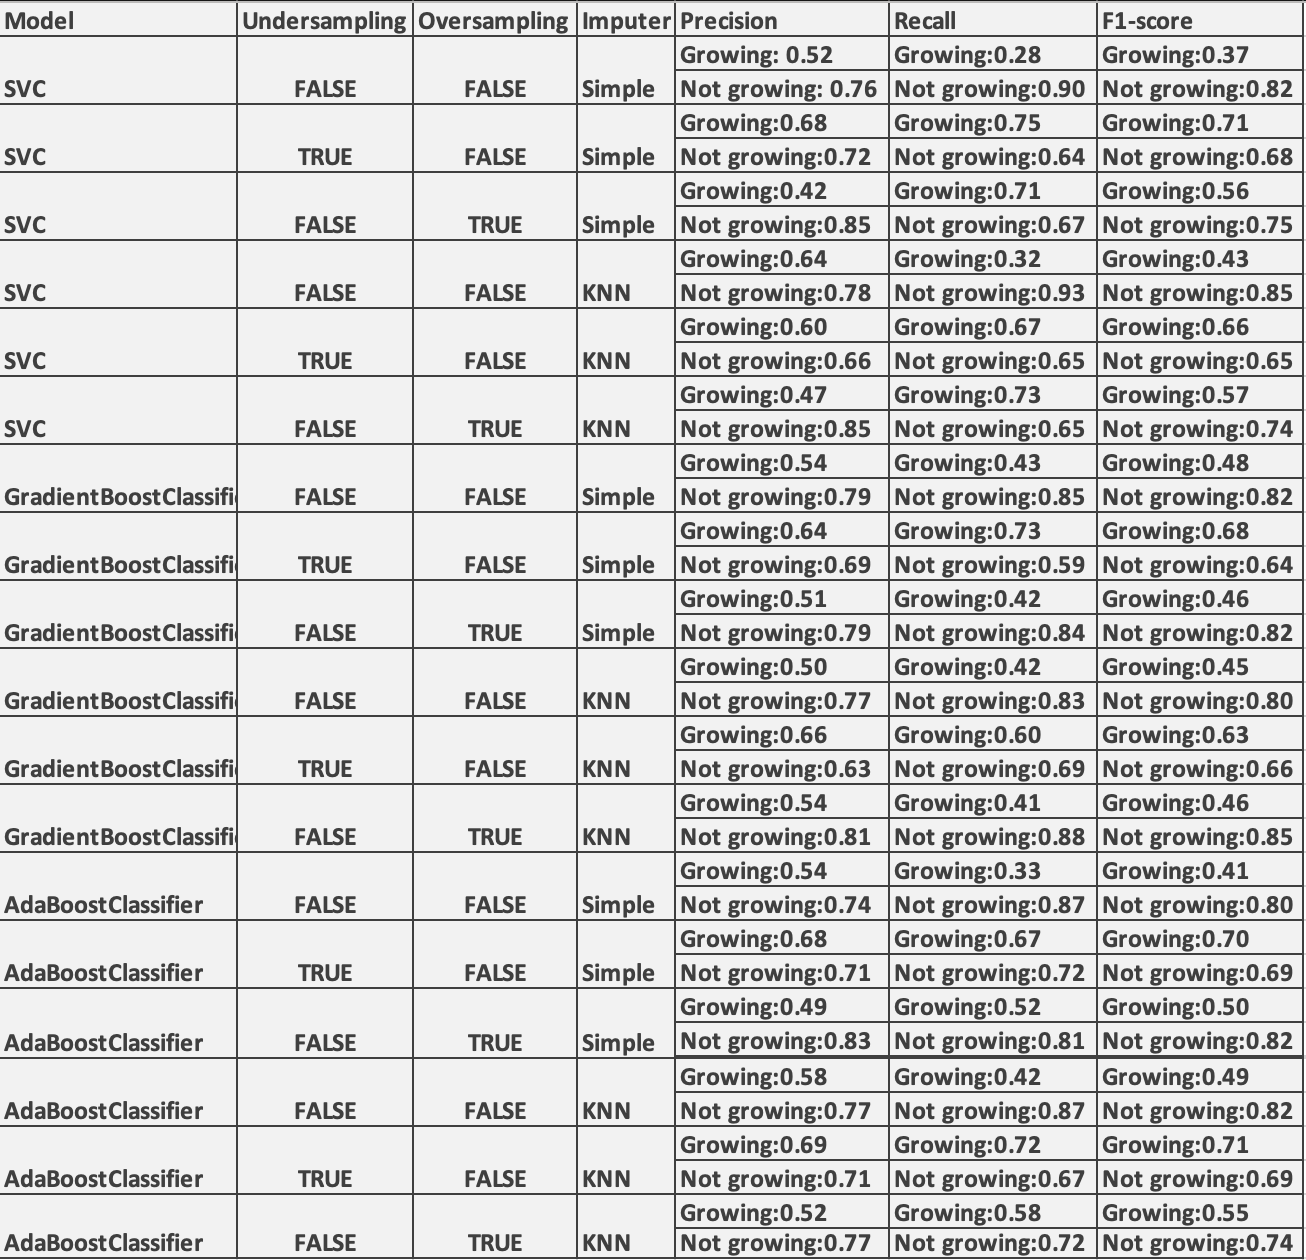
\includegraphics[scale=0.5]{results/Classifier results.png}
    \caption{Classifier performance in multiple combinations of parameters and models}
\end{figure}

The best performance was achieved using KNNImputer(\cite{scikit-learn}) on the training data, followed by oversampling via SMOTE(\cite{JMLR:v18:16-365}), using the GradientBoostClassifier(\cite{scikit-learn}), earning a respectable 76\% overall accuracy in testing, with the following report:

\begin{table}[h]
  \caption{Best performing configuration results of the classifier model}
  \label{tab:pretrained-models}
  \begin{tabularx}{\textwidth}{|X|X|X|X|X|}
    \toprule
    {}&{Precision}&{Recall}&{F1-Score}&{Support}\\
    \midrule
    False & 0.81 & 0.88 & 0.85 & 656\\\hline
                       
    True & 0.56 & 0.47 & 0.51 & 224\\\hline
    Overall \\ accuracy &  &  & 0.76 & 880\\\hline
  \bottomrule
\end{tabularx}
\end{table}

\begin{figure}[h]
    \centering
    \subfigure[a]{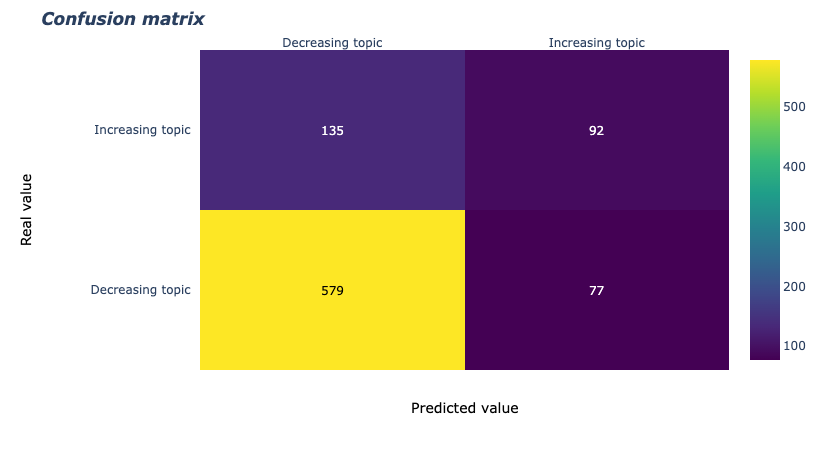
\includegraphics[width=0.45\textwidth]{results/confusion_matrix_classifier.png}} 
    \subfigure[b]{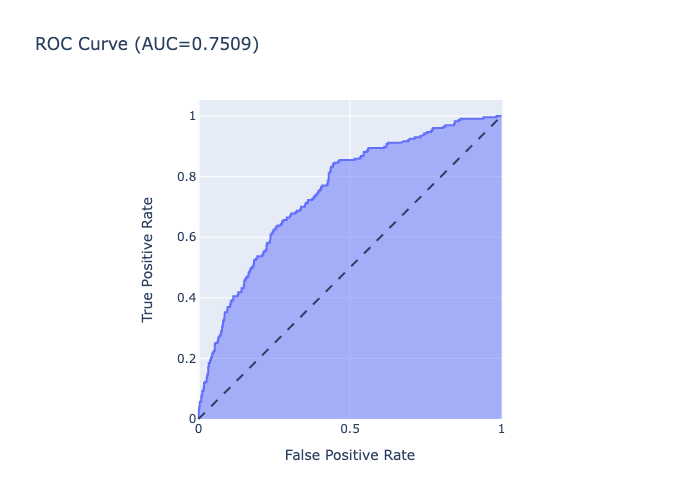
\includegraphics[width=0.45\textwidth]{results/ROC_curve_classifier.png}} 
    \caption{Visualisation of results for best performing classifier model (a) Confusion matrix (b) ROC curve}
    \label{fig:foobar}
\end{figure}

I also compared the pre-trained embeddings used to generate the DTM dataset. All the testing was performed with custom variant, custom pre-processing and the best performing parameters. spaCy did not enter this comparasion because it generated too few topics in the DTM output(15) to train and test the classifier.
\begin{table}[h]
  \caption{Pre-trained models perfomance comparasion for the classification task}
  \label{tab:pretrained-models}
  \begin{tabularx}{\textwidth}{|X|X|X|X|}
    \toprule
    {Library used}&{Precision}&{Recall}&{F1-Score}\\
    \midrule
    sentence-transformers & Growing:0.54 & Growing:0.41 & Growing:0.46 \\
    (all-mpnet-base-v2) & Not growing:0.81 & Not growing:0.88 & Not growing:0.85\\\hline
    flair & Growing:0.51 & Growing:0.50 & Growing:0.51 \\
    (all-mpnet-base-v2) & Not growing:0.84 & Not growing:0.84 & Not growing:0.84\\\hline
    tensorflow\_hub & Growing:0.46 & Growing:0.47 & Growing:0.46 \\
    USE & Not growing:0.82 & Not growing:0.81 & Not growing:0.81\\\hline
  \bottomrule
\end{tabularx}
\end{table}

\section{Regression Results}
The regression model performed respectably well after hyperparameter tunning. For a more in-depth overview of the logs regarding it and the results, you can look at the appendix (\ref{appendix:13} 13). 
During implementation, I experimented with using MACD, but it did not add enough value to be kept. The final features-target value correlation heatmap can be analysed underneath:
\begin{figure}[h]
    \centering
    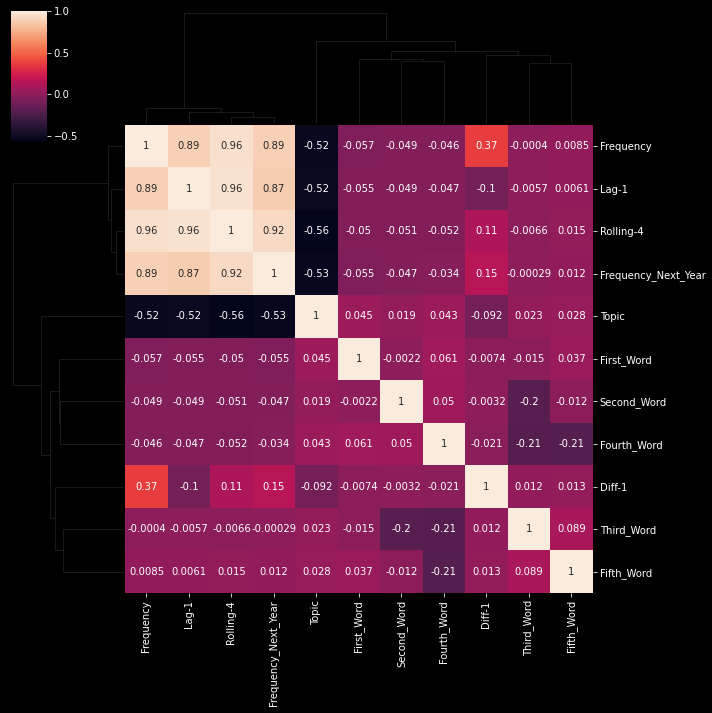
\includegraphics[scale=0.25]{regression_features_corellation.png}
    \caption{Features - target value correlation heatmap}
\end{figure}

Frequency, Lag-1 and Rolling-4 were highly correlated, as expected. The embeddings of the most representative tokens had a minor impact on the overall performance.

The following table shows the best performances achieved in each of the three experiments. The exact configuration was used for getting it for these experiments for all three libraries used. spaCy was excluded directly due to the very few data points, which made the results inconclusive:

\begin{table}[h]
  \caption{Pre-trained models perfomance comparasion for the regression task}
  \label{tab:pretrained-models}
  \begin{tabularx}{\textwidth}{|C|C|L|C|C|C|C|}
    \toprule
    {Library used}&{Experiment}&{Outliers(frequency \textgreater25)}&{RMSE}&{MAE}&{MAPE}&{R2}\\
    \midrule
    sentence-transformers & 1 & With & 1.40 & 0.86 & 46.17\% & 0.70\\
    sentence-transformers & 1 & Without & 1.25 & 0.83 & 45.21\% & 0.63\\
    sentence-transformers & 2 & With & 2.51 & 1.20 & 38.88\% & 0.72\\
    sentence-transformers & 2 & Without & 1.85 & 1.10 & 38.21\% & 0.59\\
    sentence-transformers & 3 & With & 1.37 & 0.83 & 45.21\% & 0.73\\
    sentence-transformers & 3 & Without & 1.22 & 0.80 & 43.93\% & 0.64\\
    flair & 1 & With & 1.19 & 0.79 & 45.35\% & 0.50\\
    flair & 1 & Without & 1.13 & 0.79 & 46.11\% & 0.47\\
    flair & 2 & With & 1.98 & 1.08 & 42.08\% & 0.43\\
    flair & 2 & Without & 1.69 & 1.04 & 42.01\% & 0.43\\
    flair & 3 & With & 1.16 & 0.83 & 45.21\% & 0.73\\
    flair & 3 & Without & 1.13 & 0.80 & 43.93\% & 0.64\\
    tensorflow\_hub & 1 & With & 2.31 & 1.03 & 41.41\% & 0.88\\
    tensorflow\_hub & 1 & Without & 1.86 & 0.62 & 17.81\% & 0.92\\
    tensorflow\_hub & 2 & With & 4.93 & 1.41 & 35.33\% & 0.78\\
    tensorflow\_hub & 2 & Without & 1.74 & 1.04 & 35.01\% & 0.84\\
    tensorflow\_hub & 3 & With & 2.30 & 0.98 & 39.78\% & 0.89\\
    tensorflow\_hub & 3 & Without & 1.37 & 0.84 & 40.63\% & 0.84\\
  \bottomrule
\end{tabularx}
\end{table}

By far the best performer was the Universal Sentence Embedder using tensorflowhub. This is due to the better evolutionary tuning allowed by the high dimensional representation created during training. \\
\begin{figure}[h]
    \centering
    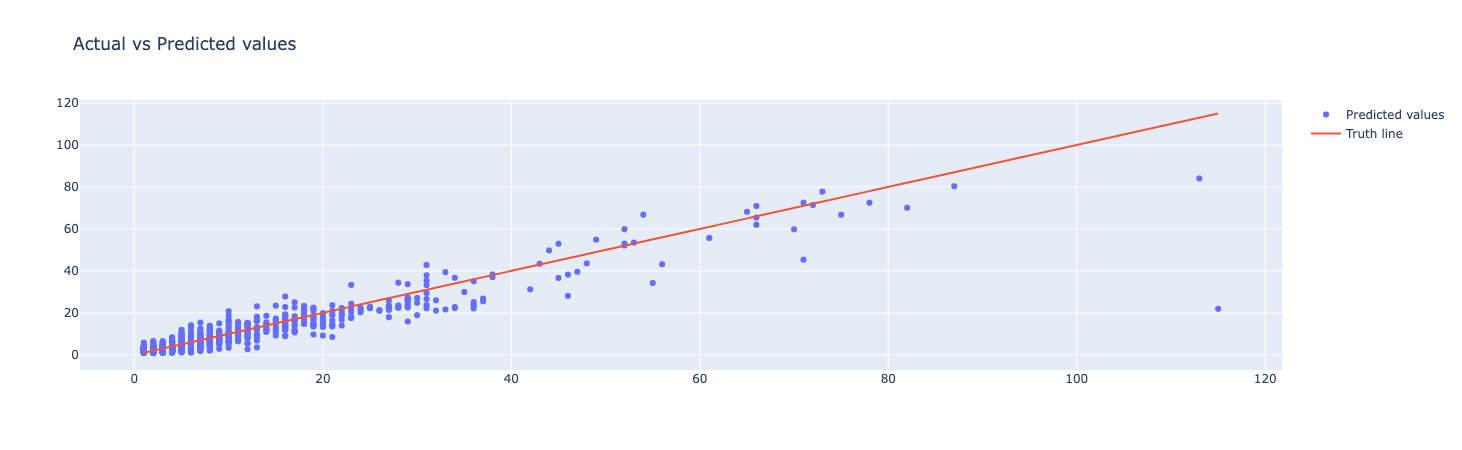
\includegraphics[scale=0.25]{results/Regression result.png}
    \caption{Actual versus Predicted plot to visualise the performance of USE regression with outliers in the dataset}
\end{figure}

The main observation is that most points are clustered in the first part of the graph, so there is very little support in training data for the later higher valued points.

This model can predict how a topic will evolve in the next year. For example, you can consult this extract of the predictions for the year 2022
\begin{figure}[h]
    \centering
    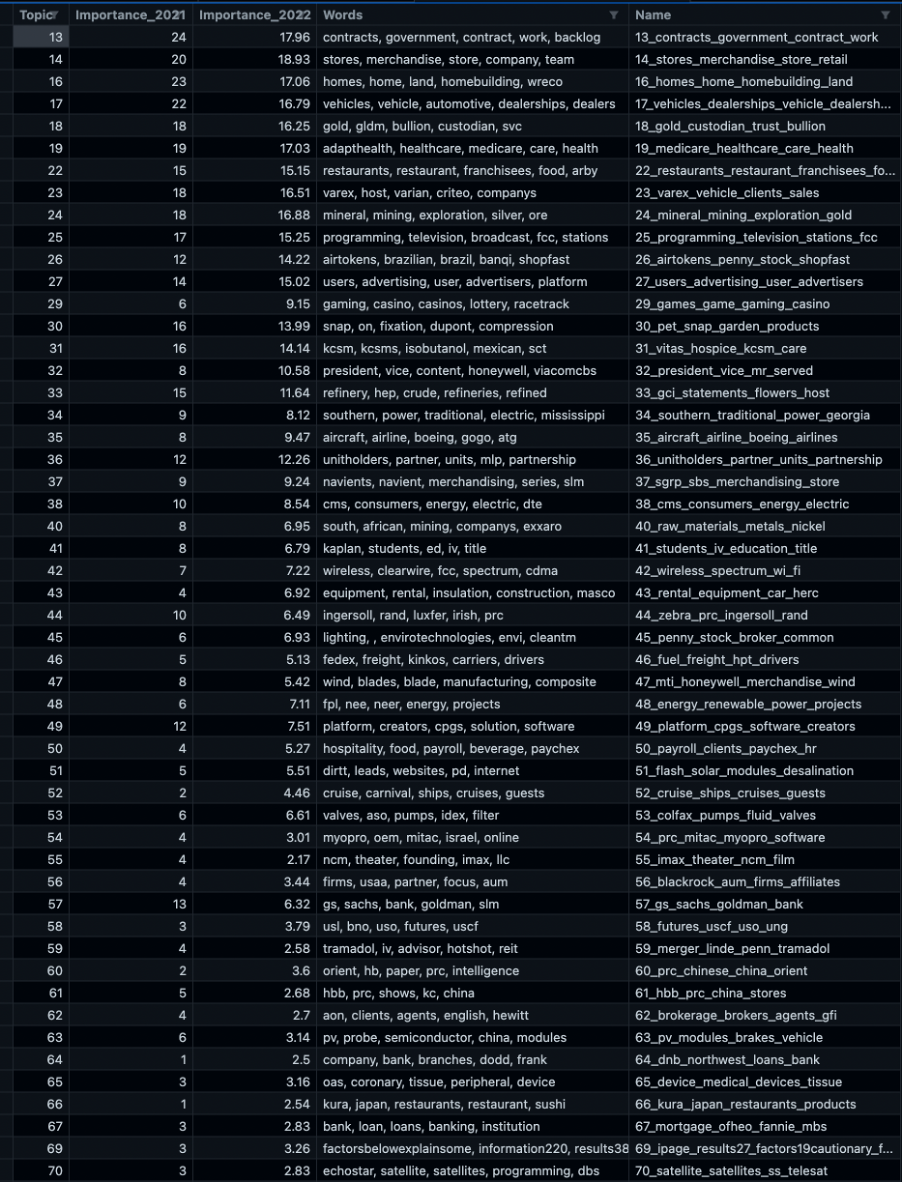
\includegraphics[scale=0.6]{results/result_regression_2022.png}
    \caption{Predicted importance for 2022}
\end{figure}


\chapter{Conclusions}

\section{Results}

Finally, we can conclude these results. The classifier and time-series predicting models did not perform well enough to be deemed acceptable. Both BERTopic and the regression model provide great insights. Topic modelling offers a pathway to extracting the essence of such a large dataset, with extensive visualisation tools and evolution tracking. The regression model can predict the importance of a particular topic with a low error rate, guiding real-world applications where knowing how a business area will develop can lead to profits.

\section{Availability}

All the data utilised in this project is publicly available and free to use (\cite{sec-data-policy}). Moreover, the object of this research is purely analytical, providing insights into documents without expressing any opinions or offering suggestions regarding investing or trading. All the libraries used in the implementation phase are public and free. Every part of the implementation taken from a different source has been linked.

\section{Limitations}

As with any research, there are certain limitations posed by the approach chosen. 
The first one refers to the information extraction procedure. The dataset analysis shows that the index-based approach can result in entire paragraphs from other sections added, representing noise for the BERTopic. The keywords used are not presented in the parsed version of the documents. The companies that are not legally bound to report risk factors are also included and extracted later in the pipeline, leading to noise influencing specific topics. 
From a data cleaning point of view, the biggest challenge was choosing an appropriate pre-processing pipeline. Even though different approaches were used, there was no definitive way in which you could compare their performance besides qualitative analysis on topic modelling model outputs and the final results of the pipeline. 
Looking further down the pipeline, one feature of BERTopic which was not thoroughly tested and exploited is the modularity of the embedding model. It allows multiple embedding models with various libraries to import and test them. Even though I tried to compare the performance and deliverables of a small subset of combinations, I did not have the computing power needed to benchmark all possible combinations properly. The main bottleneck was the size of the dataset. Utilising a smaller dataset, a random subsample of a specific size yielded drastically different results based on the subsample. Specific random subsets would quickly represent all the main topics, while others would produce topics out of meaningless words.
Moreover, all the BERTopic limitations presented in the original research paper apply(\cite{bertopic-latest-paper}). However, the most impacting one for this project was the limitation of one topic per document. Every document can have as many pages as it originally had in this pipeline. There was an idea of splitting the documents into multiple paragraphs, each considered a new document and running BERTopic on that. However, the computing power constraints would be felt even further in that case.
Another downside of the pipeline proposed is the regression approach. Due to limited examples in related research, there was no straightforward approach to short-lived time-series forecasting. The pipeline has three models for the best results instead of specialising and tuning one. Moreover, the features engineered were based on the limited amount of data provided by the DTM analysis. There is potential to enhance them with external features extracted through separate analysis.
I consider that despite the shortcomings mentioned earlier, the pipeline proposed still bears significant results for future research.

\section{Further Improvements}
Throughout my research, I kept looking at ways to improve the results at each step, evaluating the feasibility based on an improvement to time investment ratio. Due to this process, I identified several critical areas in which this work can be improved.
First, the data mining procedure can be improved by utilising a Deep Neural Networks approach for Information Extraction \cite{Gogar2016DeepNN}. This will extract the Risk Factors section from a parsed document based on a model rather than getting the indexes of specific keywords. Moreover, most companies list their risk factors in order of importance. This could be automatically tagged and included in the features vector.
Secondly, the data cleaning process can be improved by creating a bespoke pipeline for clusters of annual statements part of the same domain. Different methods of pre-processing can impact the rest of the NLP tasks down the line, as outlined in \cite{qi-etal-2018-pre}. Moreover, a mapping between an index, like CIK, and the clusters of business domains for improving the specific vocabulary.
Thirdly, using a specific combination of sentence embedding and the NLP library can notably change the result and performance of the entire pipeline. A way to improve this variability in results would be to develop a standardised testing framework similar to SentEval(\cite{Conneau2017SupervisedLO}). Thurdermore, to properly test and compare, a powerful and flexible hardware computing system is needed to offer results promptly. It is also worth further investigating the topics extracted by BERTopic in the same way \cite{ABUHAY2018193} presented. Fourthly, the dataset can be expanded with the help of business and legal advisors, explaining particularities of each year's annual statements, critical changes in legislation and the structure of the documents. Moreover, they could also provide data from different countries, to which certain big companies, such as Samsung, report.
Finally, there are multiple ways in which the three models used after obtaining the time series formatted data can be improved. One way would be to enhance the DTM approach from the BERTopic pipeline with VF-DTM as presented by \cite{HalimaBanu2016TrendingTA}. Another way to enhance the classifier's performance is to implement all the features utilised by \cite{Tattershall2019DetectingBT} in the bursty classifier. You can either undersample the data or extend the dataset. One interesting experiment that might be worth considering for the regression model is to utilise a MARS approach (\cite{wiki:mars}) using the Orange library (\cite{JMLR:demsar13a}). The time series model implementation will be improving year on year by extending the range of the data points extracted by DTM. Moreover, the results might differ significantly by fine-tuning the DARTS model used. However, this is a time-intensive task that I did not have time to undertake.
I hope that these suggestions will guide future work in this field.

Extracting the most valuable topics from a sizeable textual database is an ongoing challenge. Hopefully, the methods used in this project will provide some direction for future research.

\section{Summary}
New perspectives on data can be acquired if we look at a big enough sample size. SEC EDGAR represents a sizable database. BERTopic is a fast and informative way to extract topics. DTM takes those topics and tracks their evolution through time. From there, even though the
data is still in its incipient state, we can provide time-series analysis and forecasting, leading to the results aforementioned. Moreover, we can apply a regression model to predict the importance of the topic in the following year with reasonable accuracy. It proves that working
with NLP tasks can be achieved very labour-intensive tasks such as information extraction or clustering. It uses a machine learning model to take that data and provide trend forecasting. This pipeline utilises a state of the art technique and offers a framework upon which future tools can be built. This project shows how to surface valuable insight into risk topics of businesses. These insights can provide warning signs for investors, opportunities for traders or other professionals and underline the significant themes.



\providecommand{\harvardpreambledefs}[1]{#1}
\providecommand{\harvardpreambletext}[1]{}
\bibliographystyle{dcu} %dcu
\cleardoublepage
\phantomsection\addcontentsline{toc}{chapter}{Bibliography}
\bibliography{sample-bibliography}

% Comment the following THREE lines if you do NOT have an Appendix
\appendix
\chapter{Pre-processing}
\label{appendix:1}
\begin{figure}[h]
    \centering
    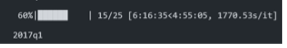
\includegraphics[scale=3]{images/appendix/Time taken by one quarter.png}
    \caption{Time taken by one quarter during data gathering utilising manual extraction.}
\end{figure}

\begin{algorithm}
\caption{Index based algorithm for extracting risk factor section}
\label{appendix:2}
\begin{algorithmic}
ids\_list = [] \newline
with open(filename) as f: \newline
     text = f.read() \newline
  pos\_1a = [m.start() for m in re.finditer('Item 1A', text)] \newline
  pos\_1b = [m.start() for m in re.finditer('Item 1B', text)] \newline
  fragments = \{\} \newline
  index\_pos1a = 0 \newline
  index\_pos1b = 0 \newline
while index\_pos1a \leq len(pos\_1a)   \&   index\_pos1b \leq len(pos\_1b): \newline
     pos1a = pos\_1a[index\_pos1a] \newline
     pos1b = pos\_1b[index\_pos1b] \newline
       if pos1a * upl\_text \leq pos1b: \newline
           index\_pos1a += 1 \newline
           continue \newline
       if pos1a \geq pos1b: \newline
           index\_pos1b += 1 \newline
           continue \newline
       fragments[(pos1a, pos1b)] = text[pos1a:pos1b] \newline
       index\_pos1a += 1 \newline
       index\_pos1b += 1 \newline
\end{algorithmic}
\end{algorithm}

\label{appendix:3}
\begin{figure}[h]
    \centering
    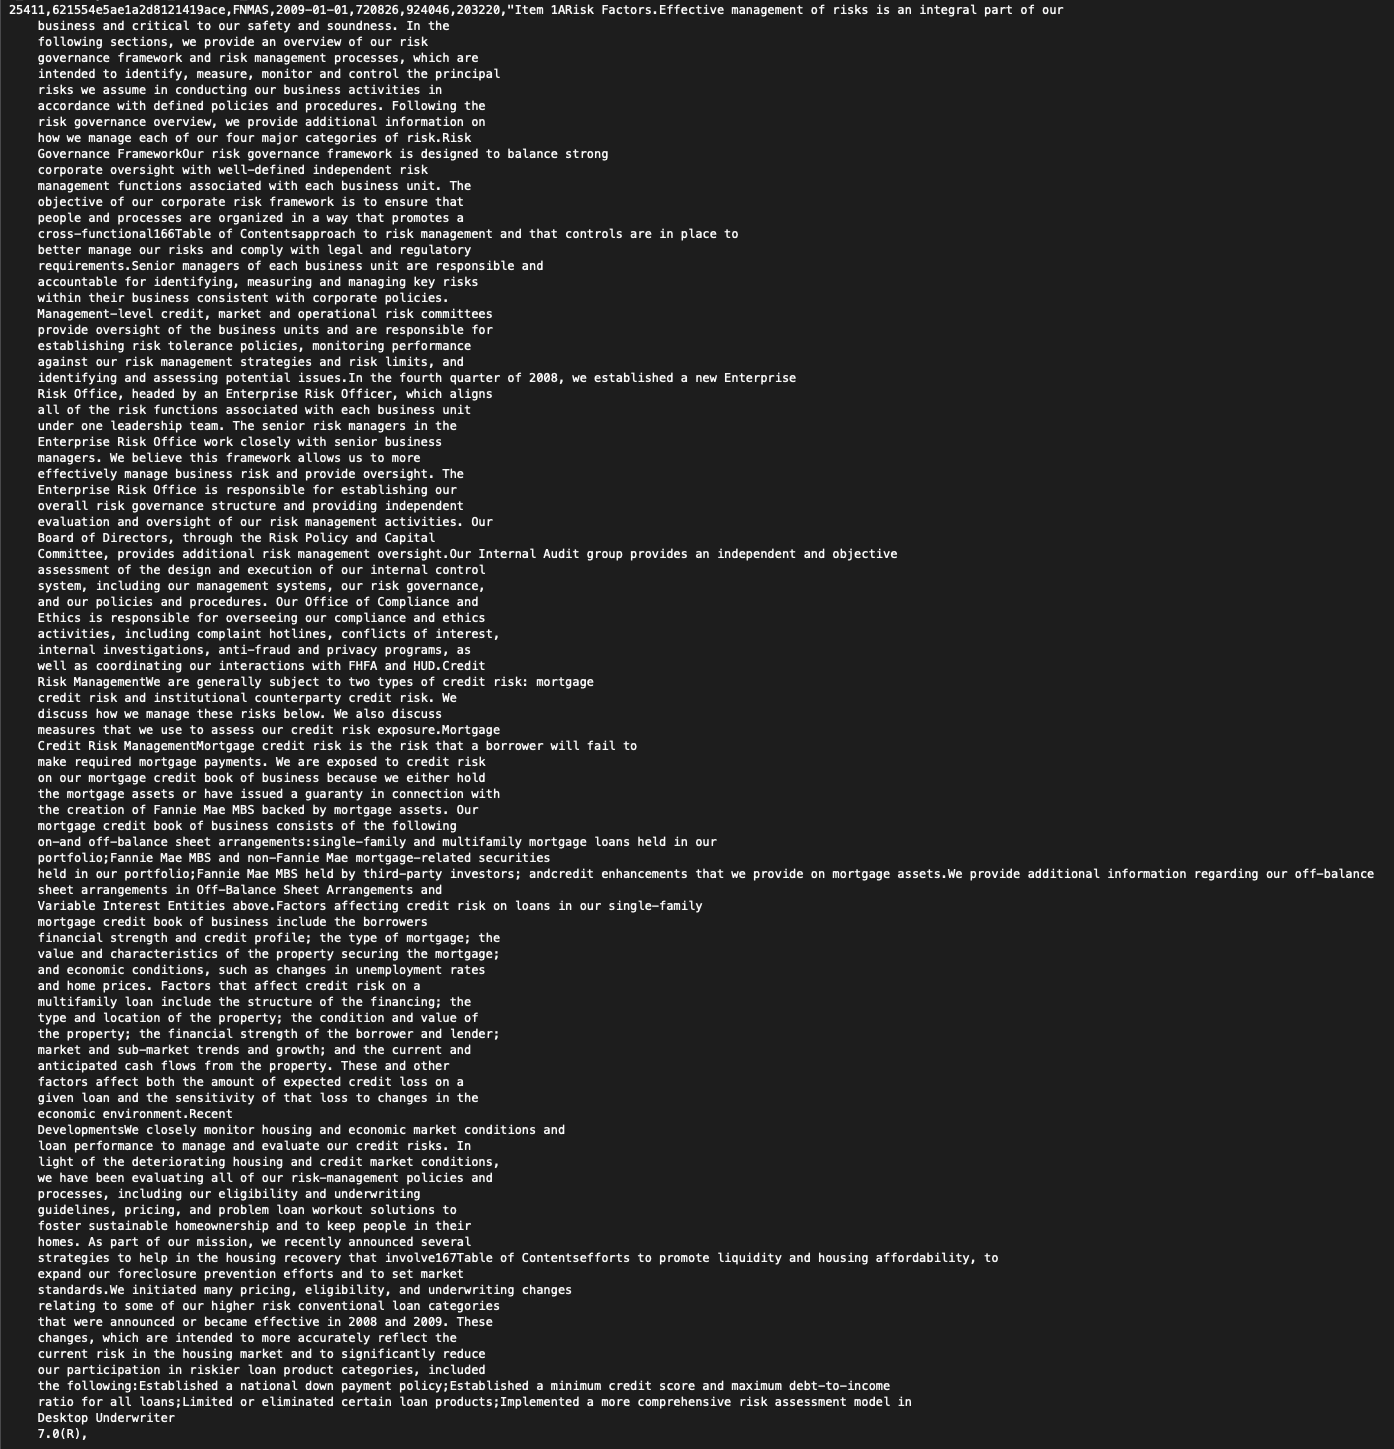
\includegraphics[scale=0.25]{images/master_tabular_file.png}
    \caption{Master tabular file}
\end{figure}

\label{appendix:4}
\begin{figure}[h]
    \centering
    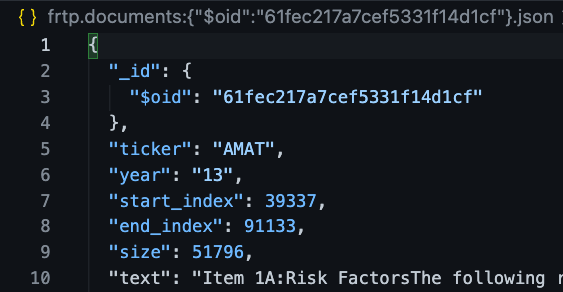
\includegraphics[scale=0.7]{images/erroneous_token.png}
    \caption{Example of erroneous extraction}
\end{figure}

\label{appendix:5}
\begin{figure}[h]
    \centering
    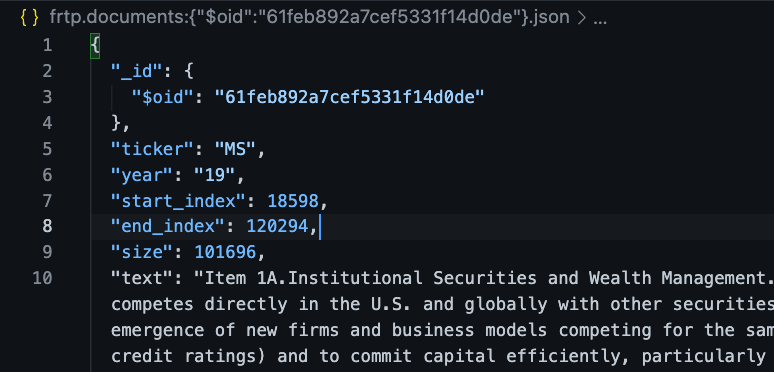
\includegraphics[scale=0.5]{images/fragment extracted.png}
    \caption{Example of a fragment extracted was considered a risk factor, but it was just a reference to the desired item.}
\end{figure}

\label{appendix:6}
\begin{figure}[h]
    \centering
    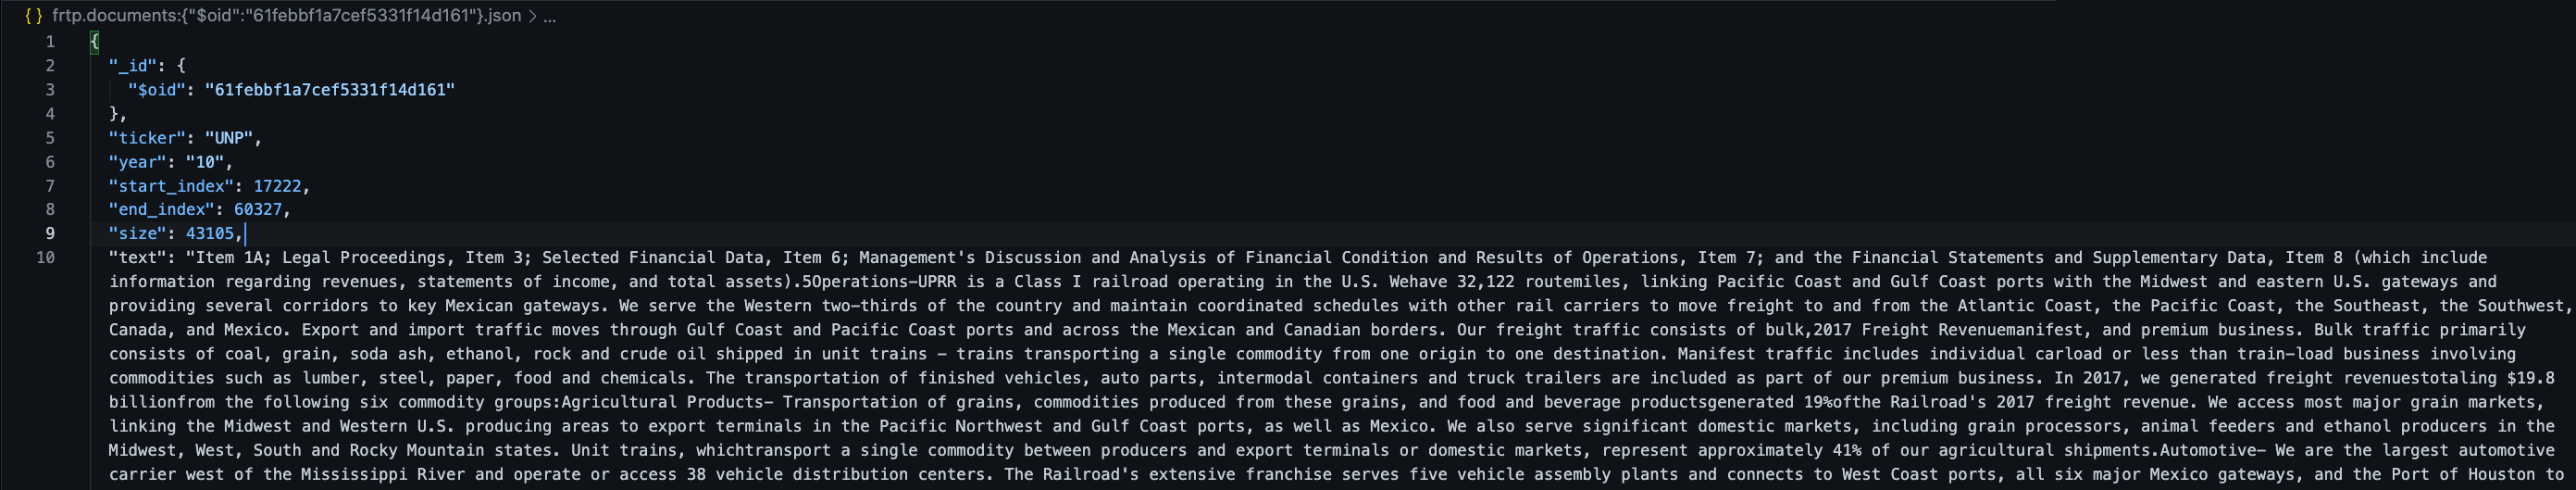
\includegraphics[scale=0.10]{images/example.png}
    \caption{Example of table of contents being extracted instead of the actual section desired}
\end{figure}

\label{appendix:7}
\begin{table}
  
  \label{tab:freq}
  \begin{tabularx}{\textwidth}{|L|X|X|X|L|}
    \toprule
    upl\_text value range & \leq8 & 8-15 (default value selected for the dataset = 10) & \textgreater 15\\
    \midrule
    Observed behaviour & Due to the early positioning of the risk factor section, the index of keyword ‘Item 1' can be \textless 1000. Testing smaller values led to ignoring lengthy sections of large companies. & Based on the subset of companies selected, this range provided the balance between ignoring smaller extracts and allowing noisy fragments. & Due to the higher value, if the risk factors section was pushed further along by structural elements or table of contents, it would lead to a very broad window from which to extract a fragment.\\
    \bottomrule
    \caption{upl\_text parameter selection options}
\end{tabularx}
\end{table}


\label{appendix:8}
\begin{figure}[h]
    \centering
    \includegraphics[scale=0.10]{images/preprocessing-sample.png}
    \caption{Sampled paragraph as testing for different pre-processing methods}
\end{figure}

\chapter{BERTopic}

\label{appendix:9}
\begin{figure}[h]
    \centering
    \includegraphics[scale=0.35]{TOT_with_global.png}
    \caption{DTM output with global tunning turned on}
\end{figure}

\label{appendix:10}
\begin{figure}[h]
    \centering
    \includegraphics[scale=0.4]{TOT_without_global.png}
    \caption{DTM output with global tunning turned off}
\end{figure}

\label{appendix:11}
\begin{figure}[h]
    \centering
    \includegraphics[scale=0.35]{images/DTM head.png}
    \caption{A head view of the DTM output produced by BERTopic}
\end{figure}

\label{appendix:12}
\begin{figure}[h]
    \centering
    \includegraphics[scale=0.3]{images/DTM Output Example.png}
    \caption{An overview of the DTM output resulting from BERTopic and how topics are tracked throughout time}
\end{figure}

\chapter{Logs}
\label{appendix:12}
\begin{figure}[h]
    \centering
    \includegraphics[scale=0.3]{results/data_gathering_log.png}
    \caption{Data Gathering log entry }
\end{figure}

\label{appendix:13}
\begin{figure}[h]
    \centering
    \includegraphics[scale=0.5]{results/regression_log.png}
    \caption{RandomForrestRegressor logging system for hyper-parameter tunning and k fold validation}
\end{figure}

% If you need more than one appendix, then just use another \chapter command
%\chapter{Yet Another Appendix}


\end{document}

%%% Local Variables:
%%% mode: latex
%%% TeX-master: t
%%% End:
